\chapter[Evaluation of Cloud Cuts on Auger Event Data]{\centering Evaluation of Cloud Cuts on Auger Event Data \\}\label{Ch:CloudCuts}

First look into the effectiveness of the Cloud cuts on Auger Golden Hybrid data from 2004 to 2018.
I investigated the effects of removing the cloud cut from the list of quality cuts. This list includes cuts to remove events within known bad data taking periods, cuts on aerosol levels, event quality etc. Below is an example of a cuts file that is used within Auger.

This investigation was done to quantify the effects that the cloud cuts had on the data set. A question had been raised about whether the quality cuts on fitted values, Chi2 and requiring events with large gaps where doing the same job as the cloud cuts. There is a lot of uncertainty about whether a detected cloud had impacted each events.

Cloud information has large uncertainty about quantities like cloud height, distance from telescopes and timing. The timing uncertainty is due to atmospheric data being snapshots with time gaps between shots. Examples are Cloud camera scans are performed every 5 minutes. A cloud could move quite a far distance within this time.

\section{Equipment used to detect cloud over the array}

IR Cloud Cameras - Two version of IR camera has been running in tandem with the operation of the FD's. Find dates of operation

GOES Satellite data

CLF and XLF

LIDAR

\section{Method - Cloud Flags and Their Impact}

Take reconstructed Golden Hybrid events from 2004 to 2018 

Extract camera flag data.

Two set of camera flags - positive ones that say that an event has pass one of the conditions saying that these is no cloud. the negative flags say that the event has failed to pass any of the test looking for clouds. If the flag is zero then there is no cloud information available.

Four different flags - IR Cloud camera, LIDAR, GOES satellite data and something else.

Look at the histograms of Xmax distributions for data passing cloud cuts, data failing cloud cuts and combined.

\begin{figure}
\centering
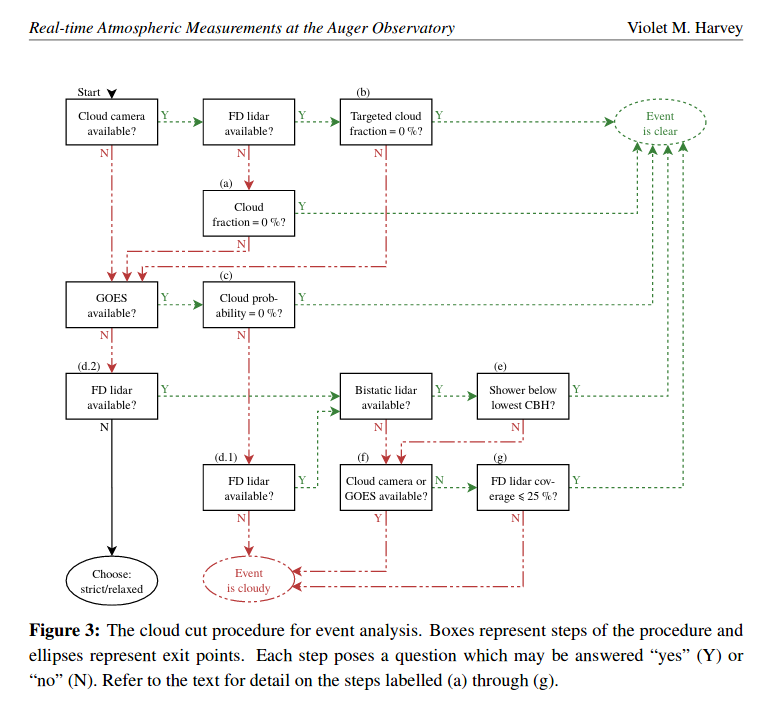
\includegraphics[width=0.7\textwidth]{chapters/pictures/Violet_ICRC2019_CloudCut_Diagram.png}
\caption{Diagram of how the cloud cuts are applied to the data set when called with the Auger event selection program.}
\end{figure}

\begin{figure}
\centering
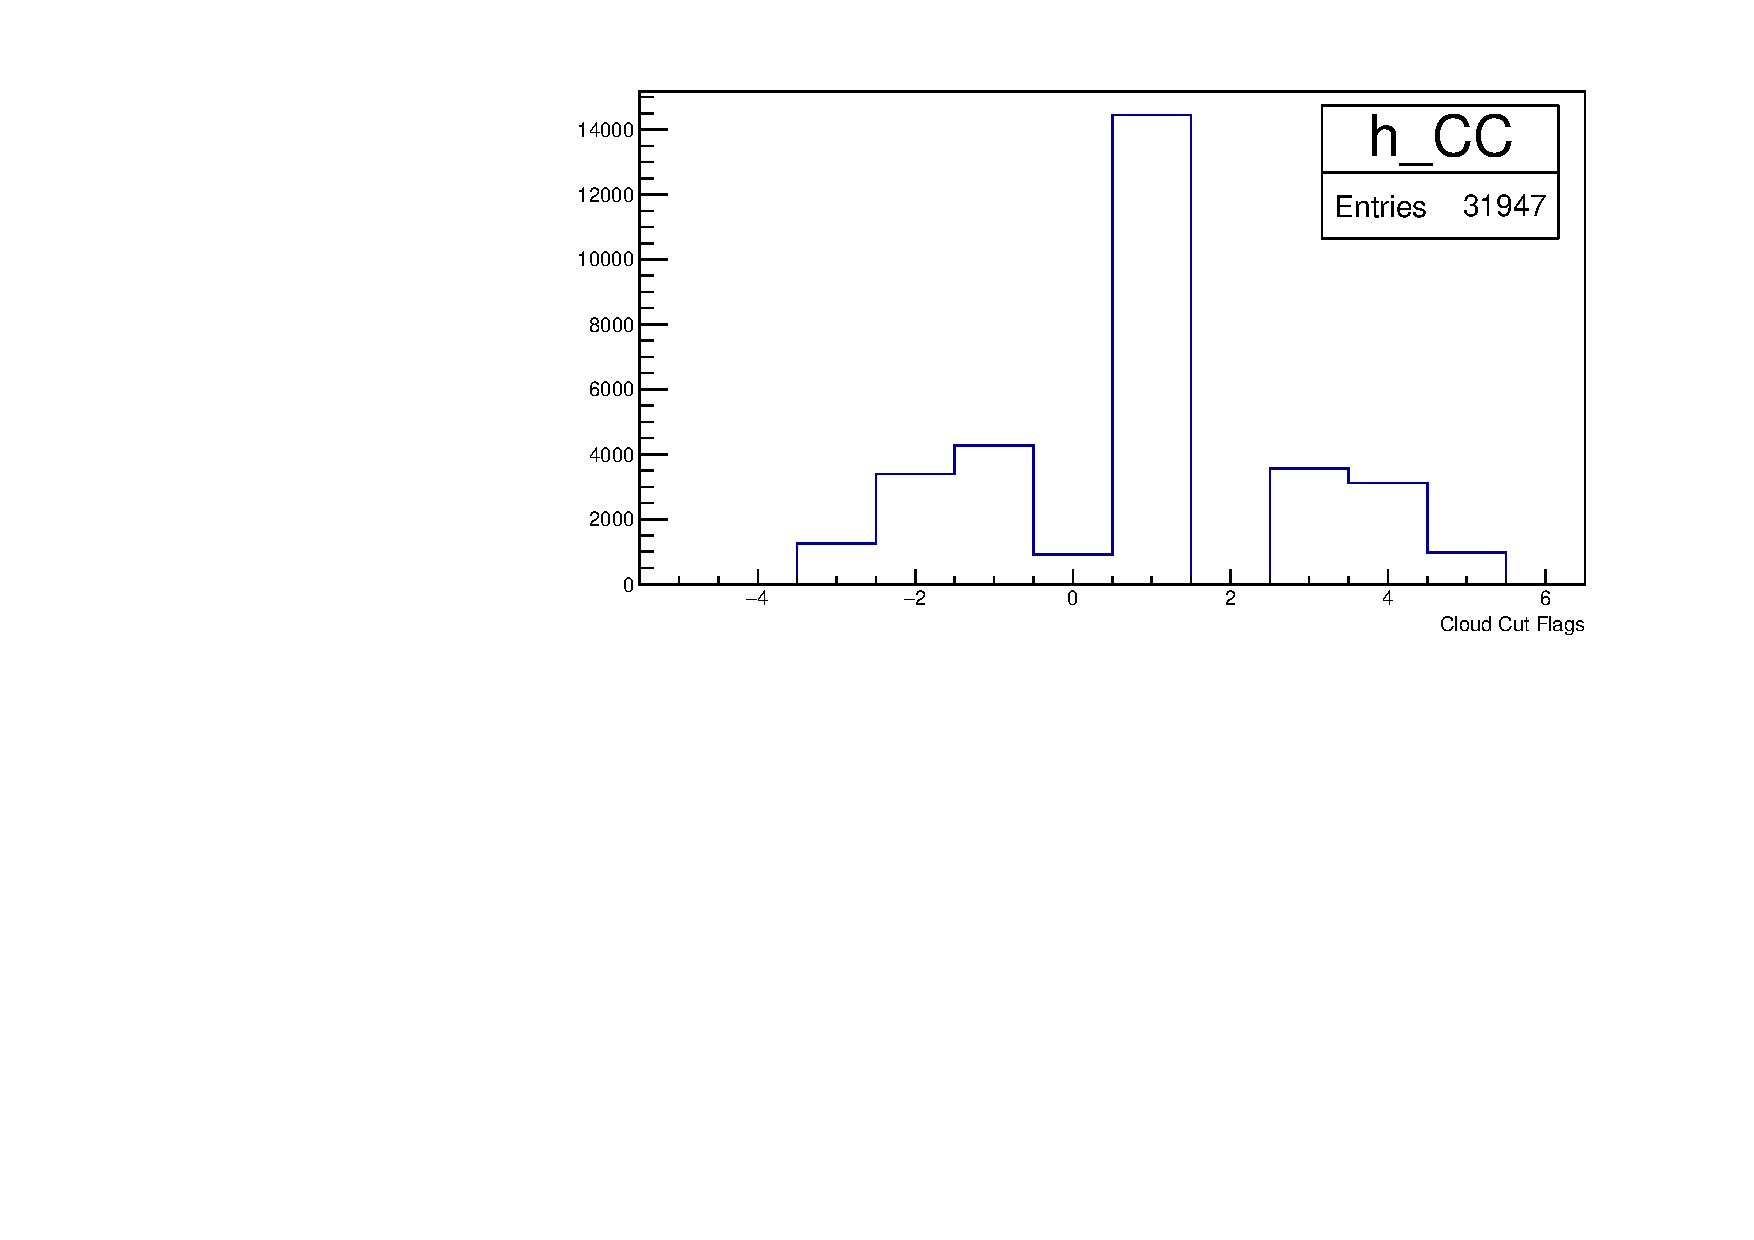
\includegraphics[width=\textwidth]{chapters/graphs/CloudFlags/hist_cloudFlags.pdf}
\caption{Distribution of cloud flags. Positive flag values are for events that would pass one of the cloud cuts. Negative flag values are for events that would one of the cloud cuts. A flag value of zero is for events that have no cloud data.}
\end{figure}

\section{Results - Effect on Mean Xmax and Spread in Xmax}

- Cloud Cut Flags distribution

- Xmax distributions within energy bins

- Elongation rate  

- Is distance to Xmax or distance to shower axis needed?

\begin{figure}
\centering
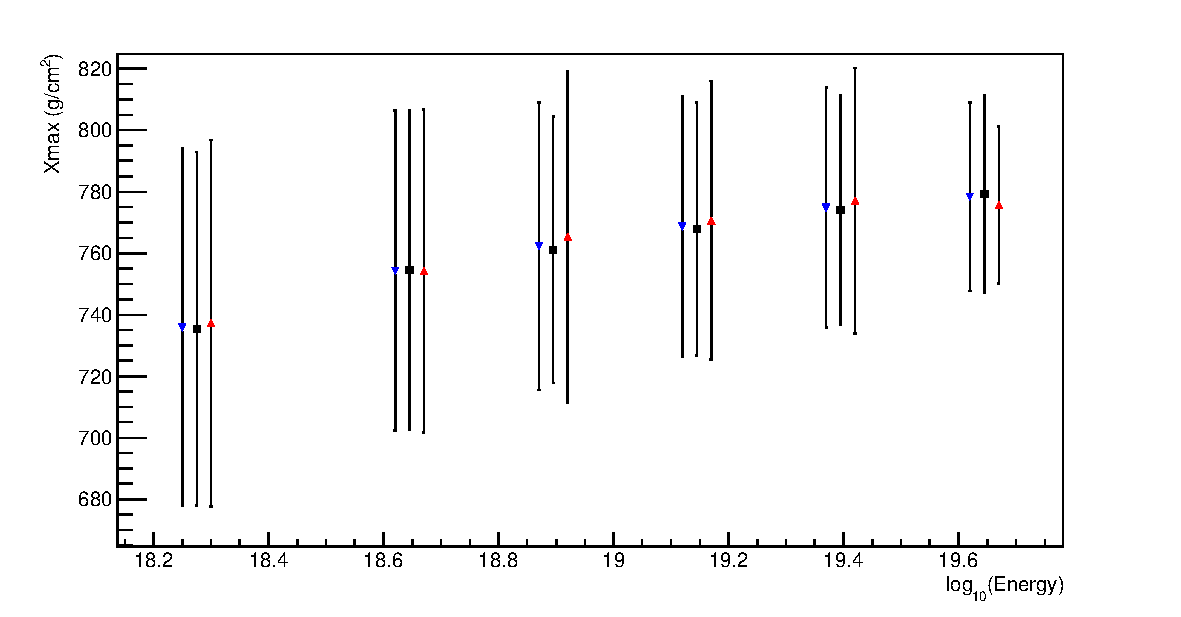
\includegraphics[width=\textwidth]{chapters/graphs/CloudFlags/ElongationRate.pdf}
\caption{Elongation Rate with Cloud cuts applied (blue downward triangle), without any cloud cuts (black square) and only events that would fail the cloud cuts (red upward triangle).}
\end{figure}

% Energy Distribution

\begin{figure}
\centering
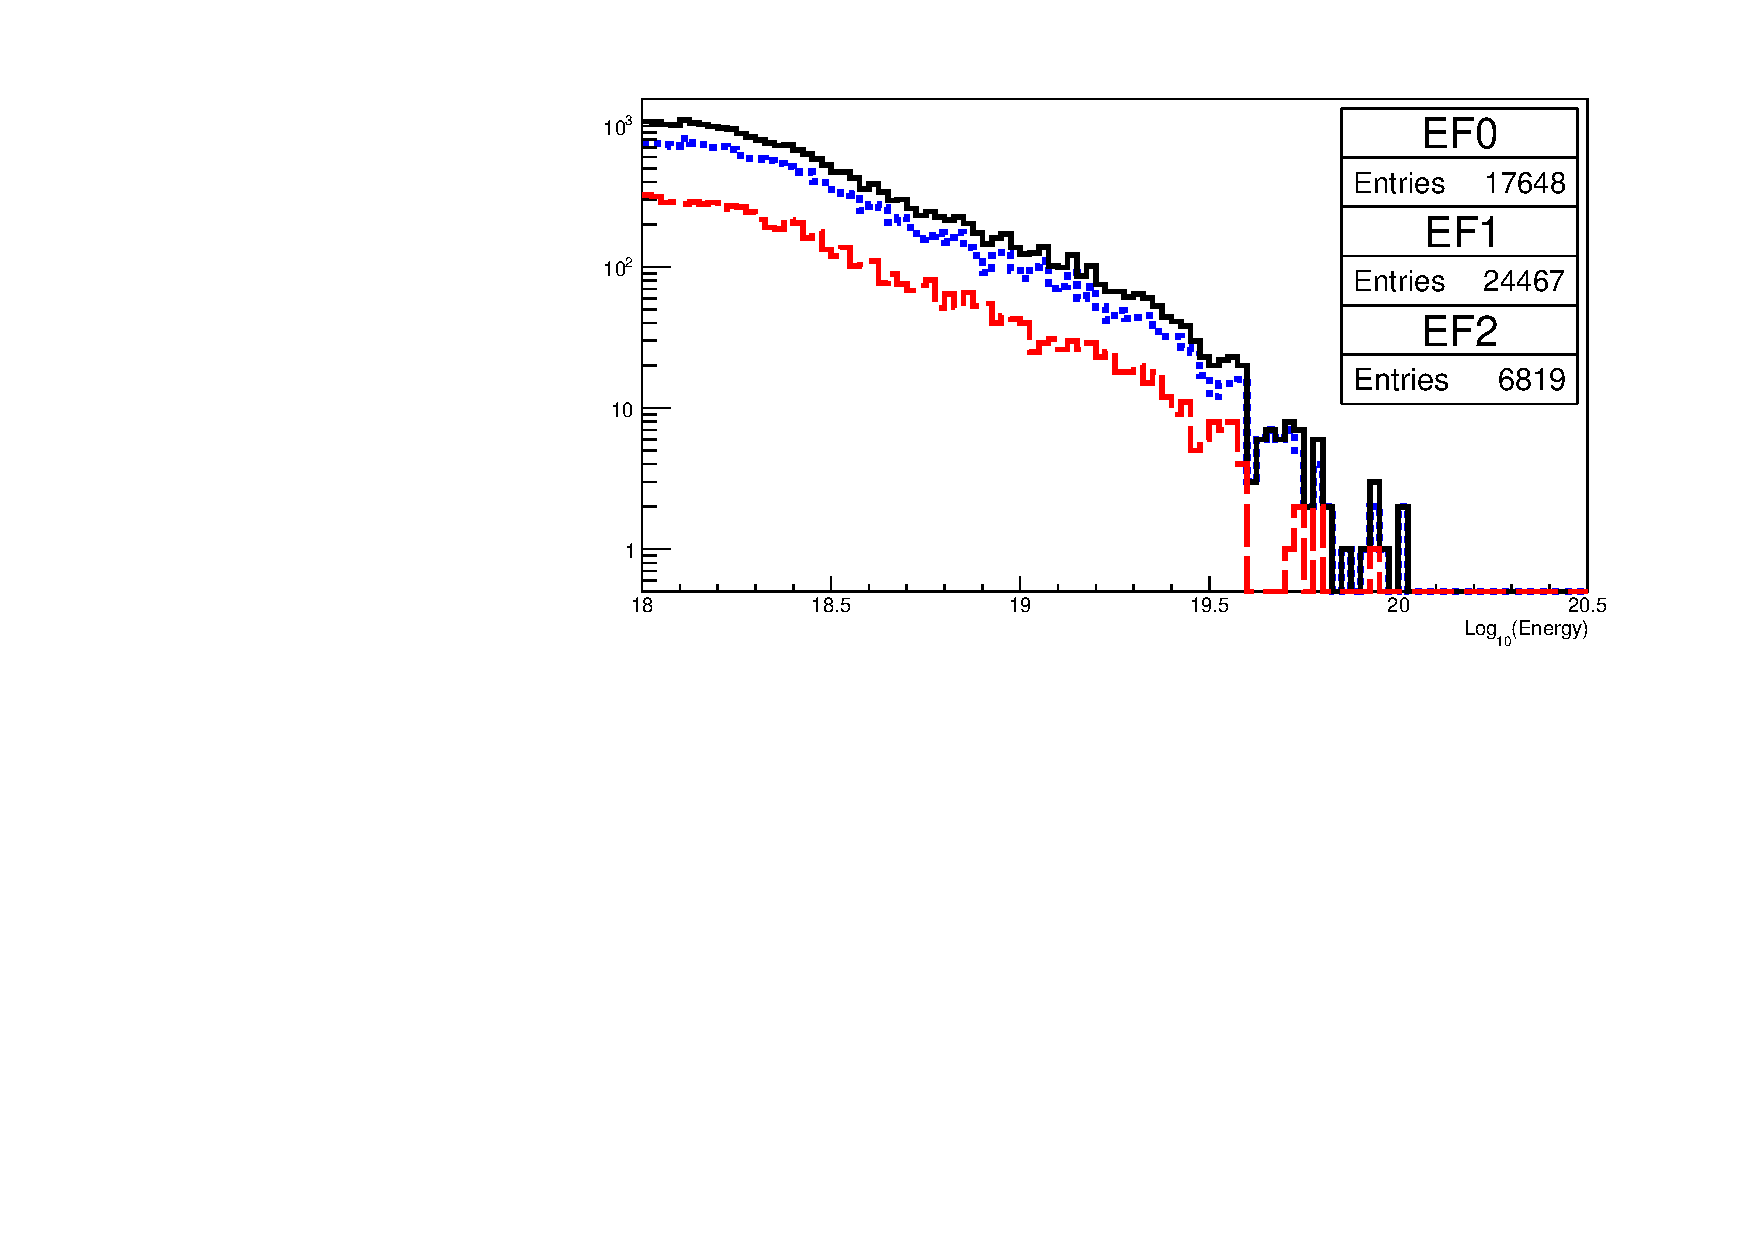
\includegraphics[width=\textwidth]{/home/tsudholz/PhD/Thesis/chapters/graphs/CloudFlags/EnergyHistAll_logE_18_0to20_5_Comb2.pdf}
\caption{Distribution of the energy of events within the bin of log(E) of 18.0 to 20.5. Black (EF1) denotes events that passed with cloud cut removed, blue (EF0) denotes events that would pass the cloud cuts and red (EF2) denotes events that would fail the cloud cuts. All other cuts used for the ICRC19 have been applied.}
\end{figure}

%\begin{figure}
%\centering
%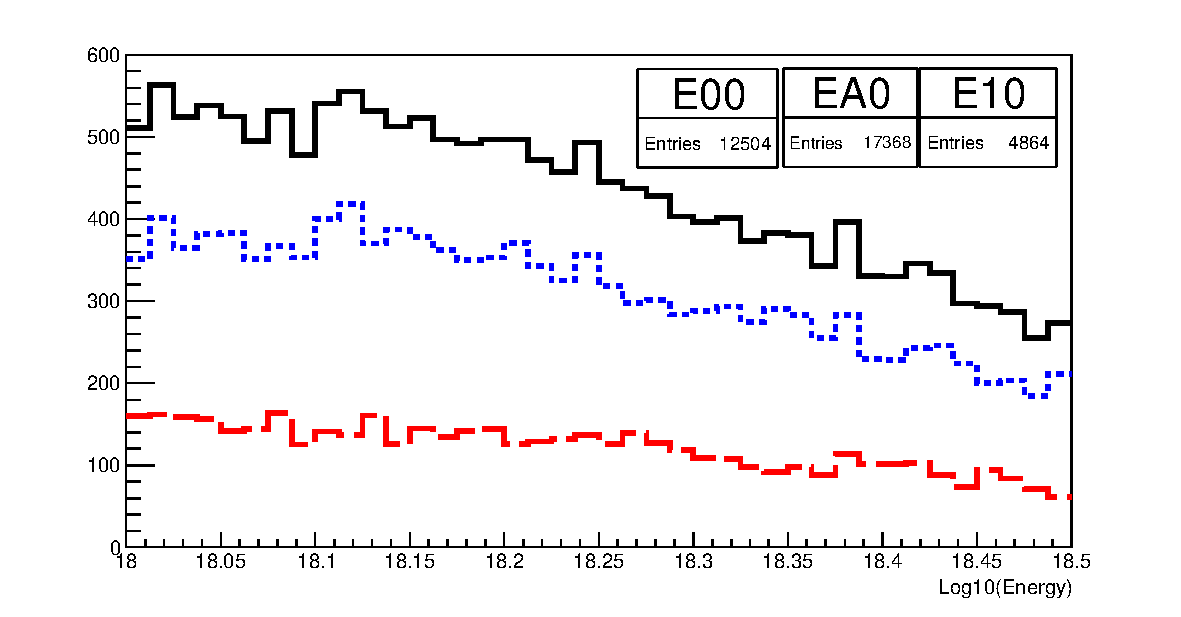
\includegraphics[width=\textwidth]{/home/tsudholz/PhD/Thesis/chapters/graphs/CloudFlags/EnergyHist_logE_18_0to18_5_Comb.pdf}
%\caption{Distribution of the energy of events within the bin of log(E) of 18.0 to 18.5. Black (EA0) denotes events that passed with cloud cut removed, blue (E00) denotes events that would pass the cloud cuts and red (E10) denotes events that would fail the cloud cuts. All other cuts used for the ICRC19 have been applied.}
%\end{figure}
%
%\begin{figure}
%\centering
%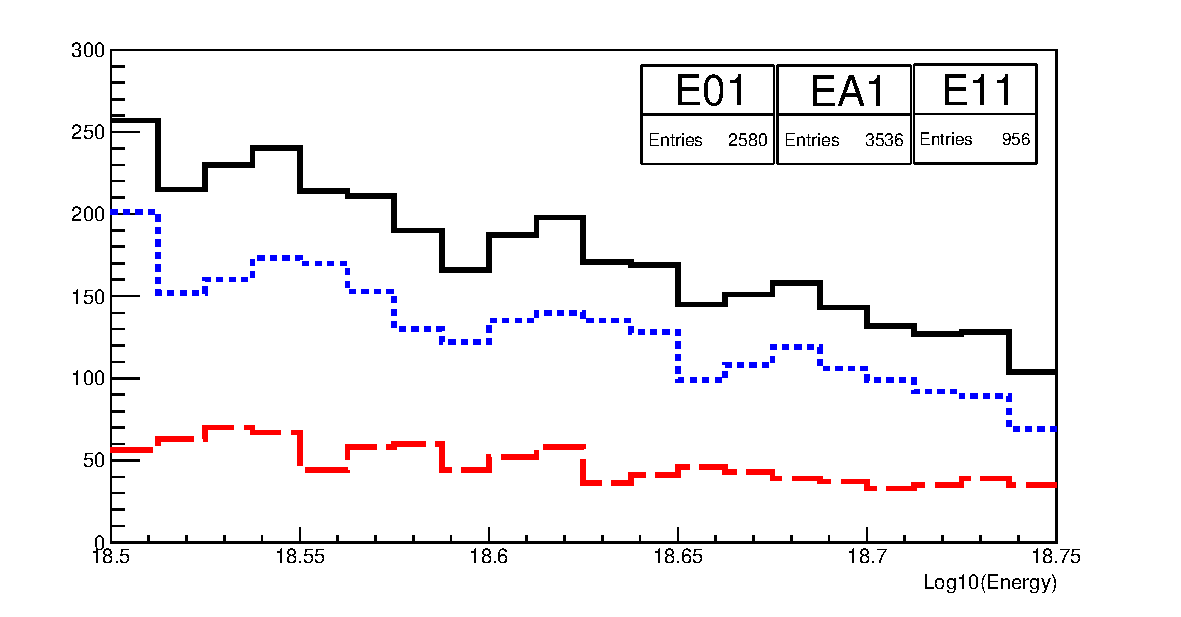
\includegraphics[width=\textwidth]{/home/tsudholz/PhD/Thesis/chapters/graphs/CloudFlags/EnergyHist_logE_18_5to18_75_Comb.pdf}
%\caption{Distribution of the energy of events within the bin of log(E) of 18.5 to 18.75. Black (EA1) denotes events that passed with cloud cut removed, blue (E01) denotes events that would pass the cloud cuts and red (E11) denotes events that would fail the cloud cuts. All other cuts used for the ICRC19 have been applied. }
%\end{figure}
%
%\begin{figure}
%\centering
%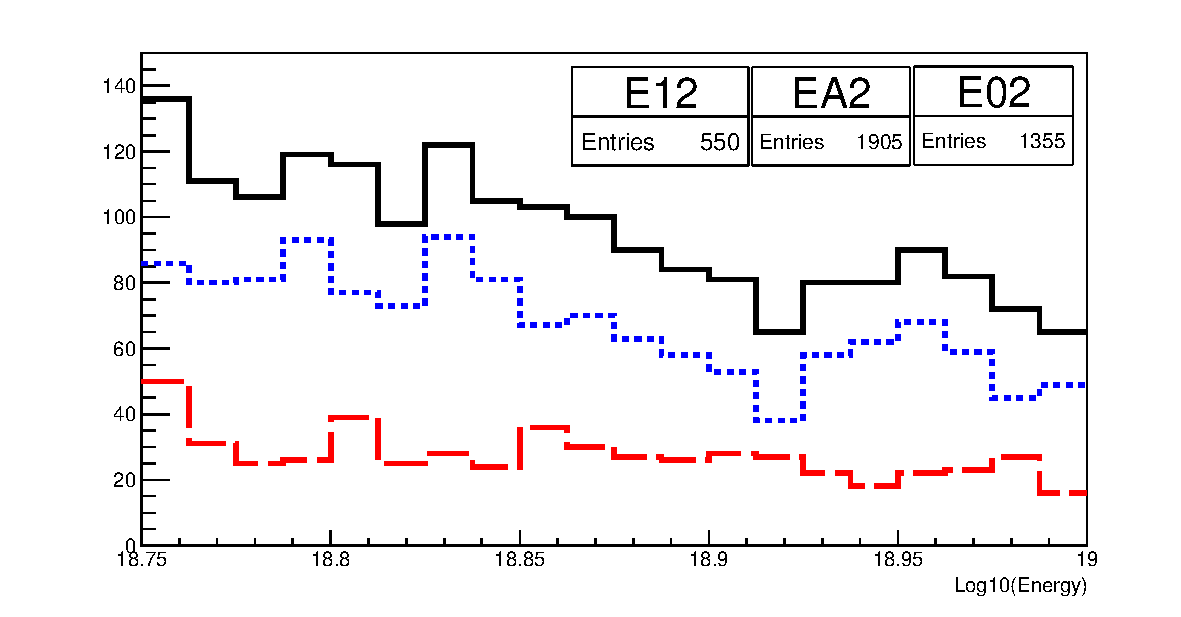
\includegraphics[width=\textwidth]{/home/tsudholz/PhD/Thesis/chapters/graphs/CloudFlags/EnergyHist_logE_18_75to19_0_Comb.pdf}
%\caption{Distribution of the energy of events within the bin of log(E) of 18.75 to 19.0. Black (EA2) denotes events that passed with cloud cut removed, blue (E12) denotes events that would pass the cloud cuts and red (E02) denotes events that would fail the cloud cuts. All other cuts used for the ICRC19 have been applied.}
%\end{figure}
%
%\begin{figure}
%\centering
%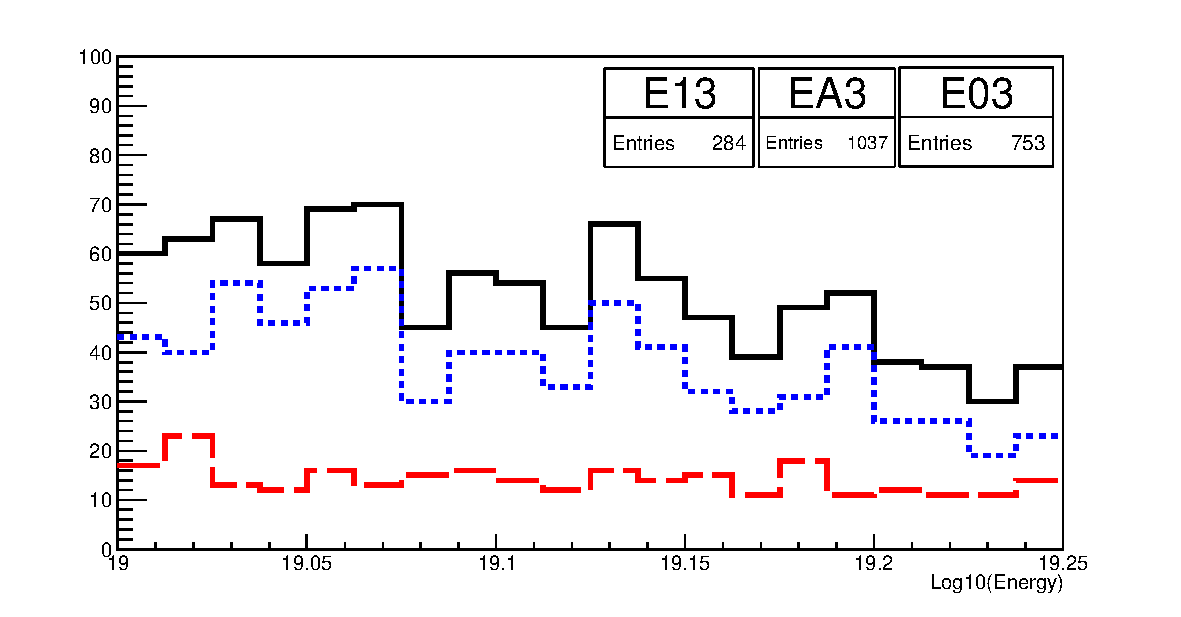
\includegraphics[width=\textwidth]{/home/tsudholz/PhD/Thesis/chapters/graphs/CloudFlags/EnergyHist_logE_19_0to19_25_Comb.pdf}
%\caption{Distribution of the energy of events within the bin of log(E) of 19.0 to 19.25. Black (EA3) denotes events that passed with cloud cut removed, blue (E13) denotes events that would pass the cloud cuts and red (E03) denotes events that would fail the cloud cuts. All other cuts used for the ICRC19 have been applied.}
%\end{figure}
%
%\begin{figure}
%\centering
%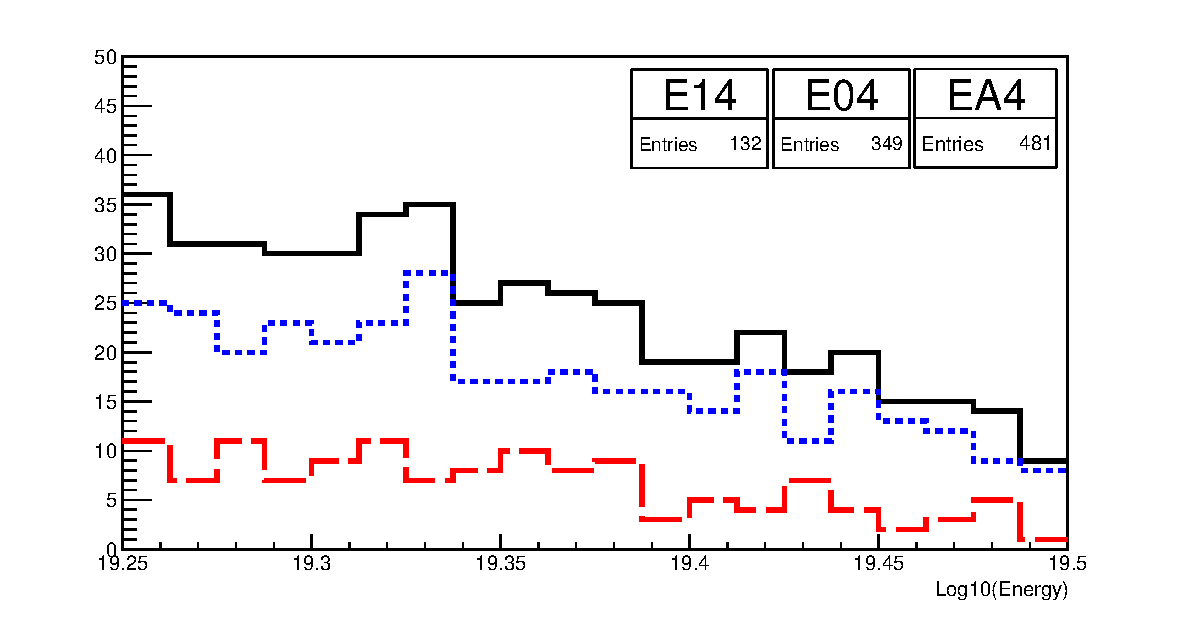
\includegraphics[width=\textwidth]{/home/tsudholz/PhD/Thesis/chapters/graphs/CloudFlags/EnergyHist_logE_19_25to19_5_Comb.pdf}
%\caption{Distribution of the energy of events within the bin of log(E) of 19.25 to 19.5. Black (EA4) denotes events that passed with cloud cut removed, blue (E14) denotes events that would pass the cloud cuts and red (E04) denotes events that would fail the cloud cuts. All other cuts used for the ICRC19 have been applied.}
%\end{figure}
%
%\begin{figure}
%\centering
%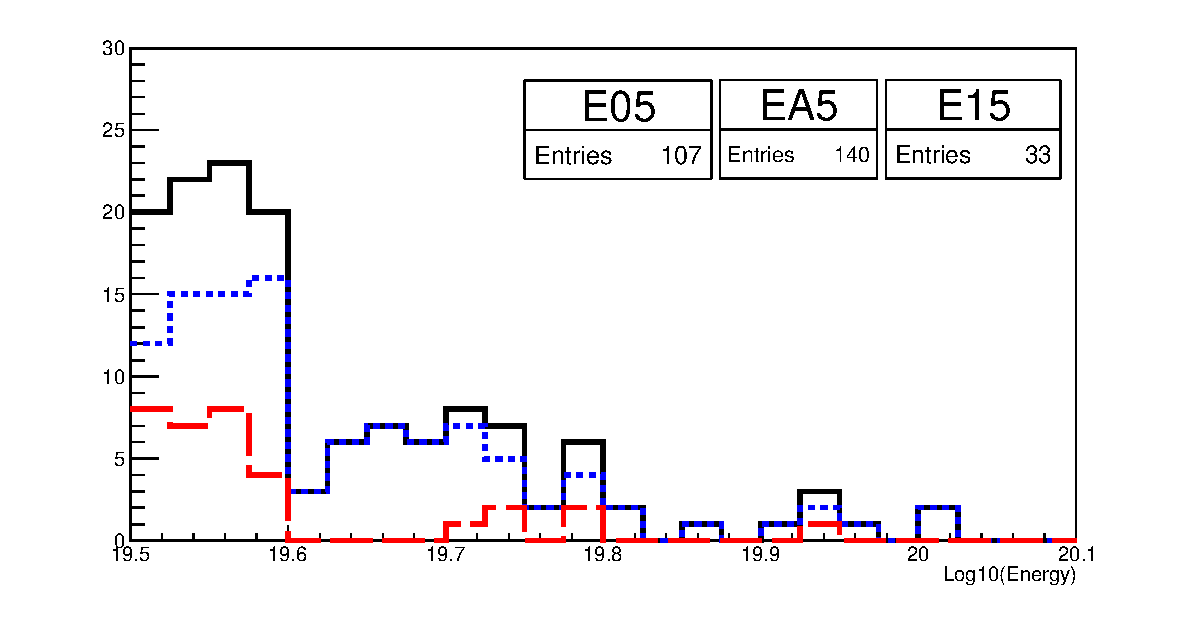
\includegraphics[width=\textwidth]{/home/tsudholz/PhD/Thesis/chapters/graphs/CloudFlags/EnergyHist_logE_Greater19_5_Comb.pdf}
%\caption{Distribution of the energy of events within the bin of log(E) of greater than 19.5. Black (EA5) denotes events that passed with cloud cut removed, blue (E15) denotes events that would pass the cloud cuts and red (E05) denotes events that would fail the cloud cuts. All other cuts used for the ICRC19 have been applied.}
%\end{figure}

% Xmax Distribution for Passed, Combined, Failed

\begin{figure}
\centering
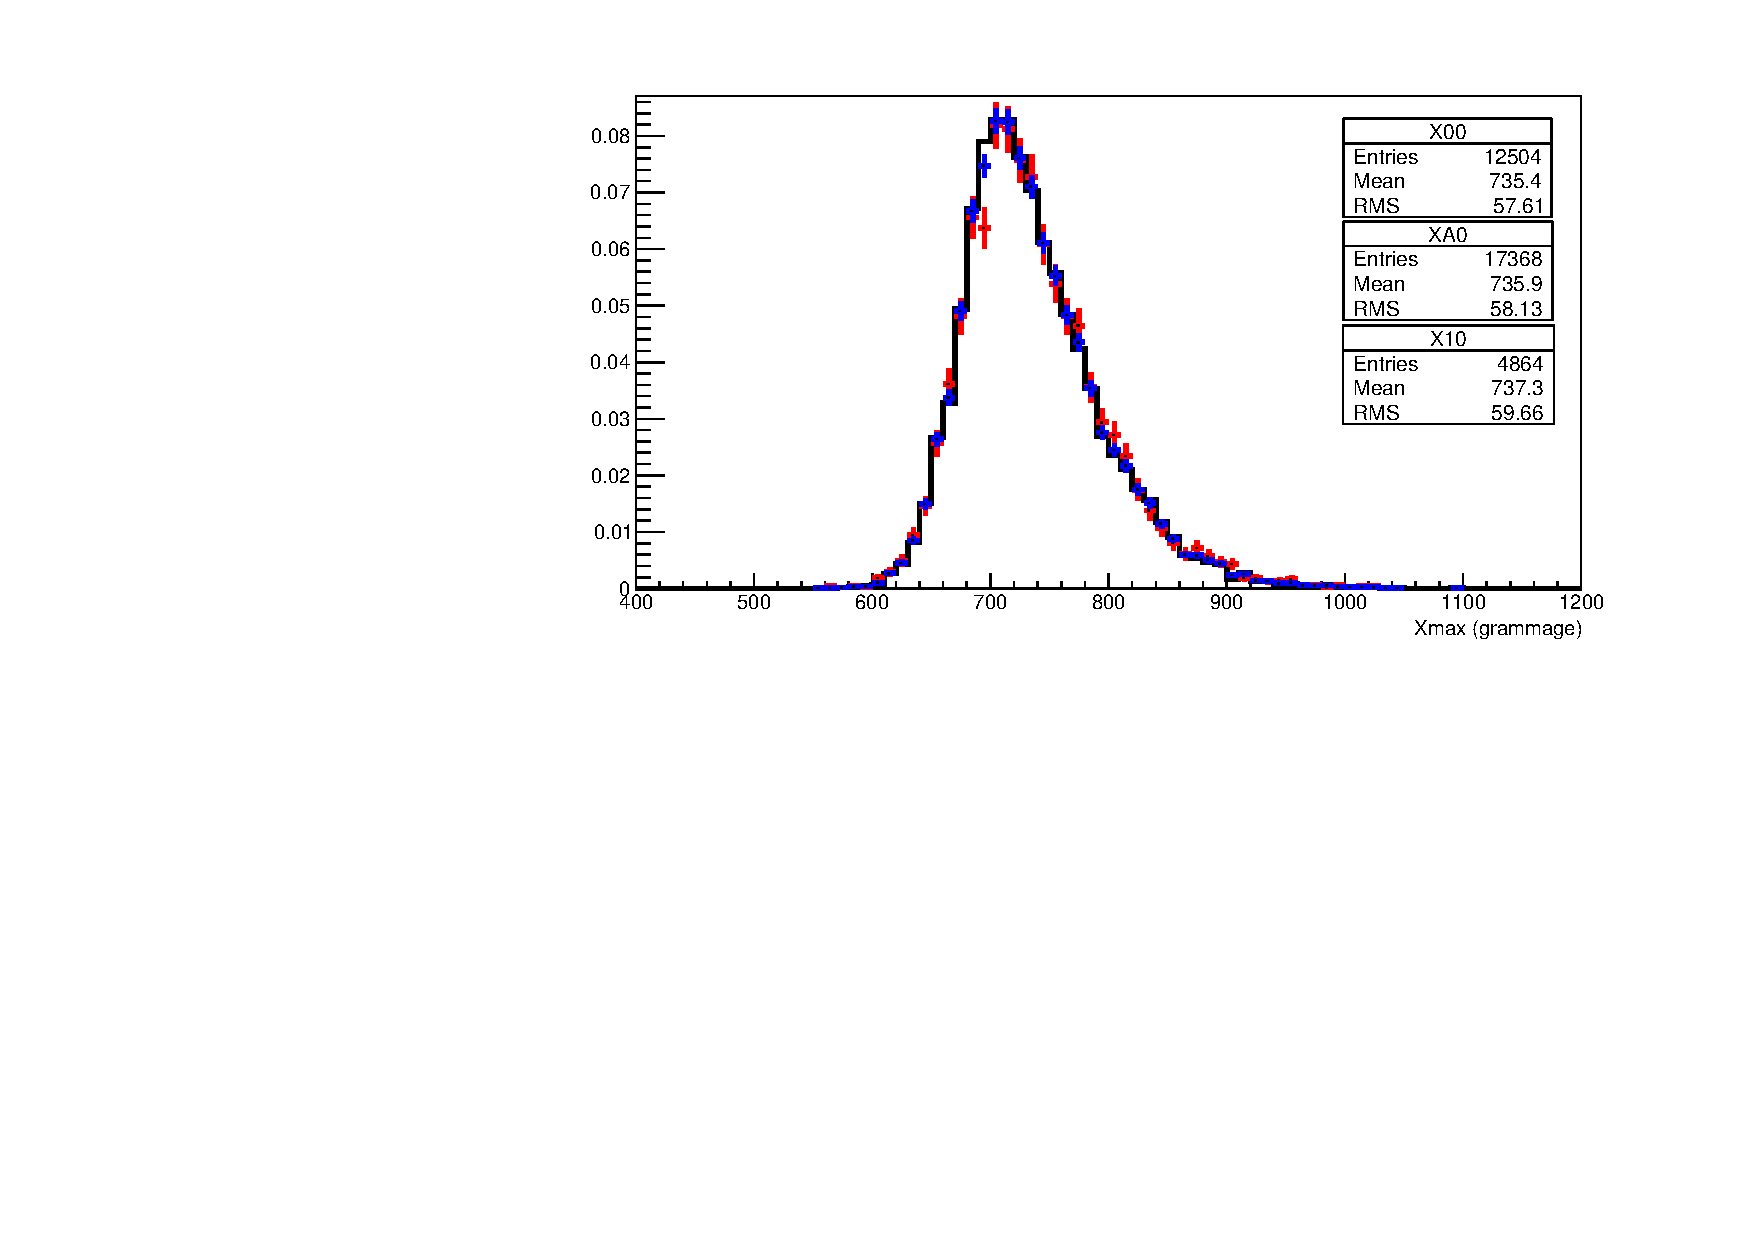
\includegraphics[width=\textwidth]{/home/tsudholz/PhD/Thesis/chapters/graphs/CloudFlags/NormHist_Xmax_logE_18_0to18_5_Comb.pdf}
\caption{Distribution of the Xmax of events within the bin of log(E) of 18.0 to 18.5. Black (XA0) denotes events that passed with cloud cut removed, blue (X00) denotes events that would pass the cloud cuts and red (X10) denotes events that would fail the cloud cuts. All other cuts used for the ICRC19 have been applied.}
\end{figure}

\begin{figure}
\centering
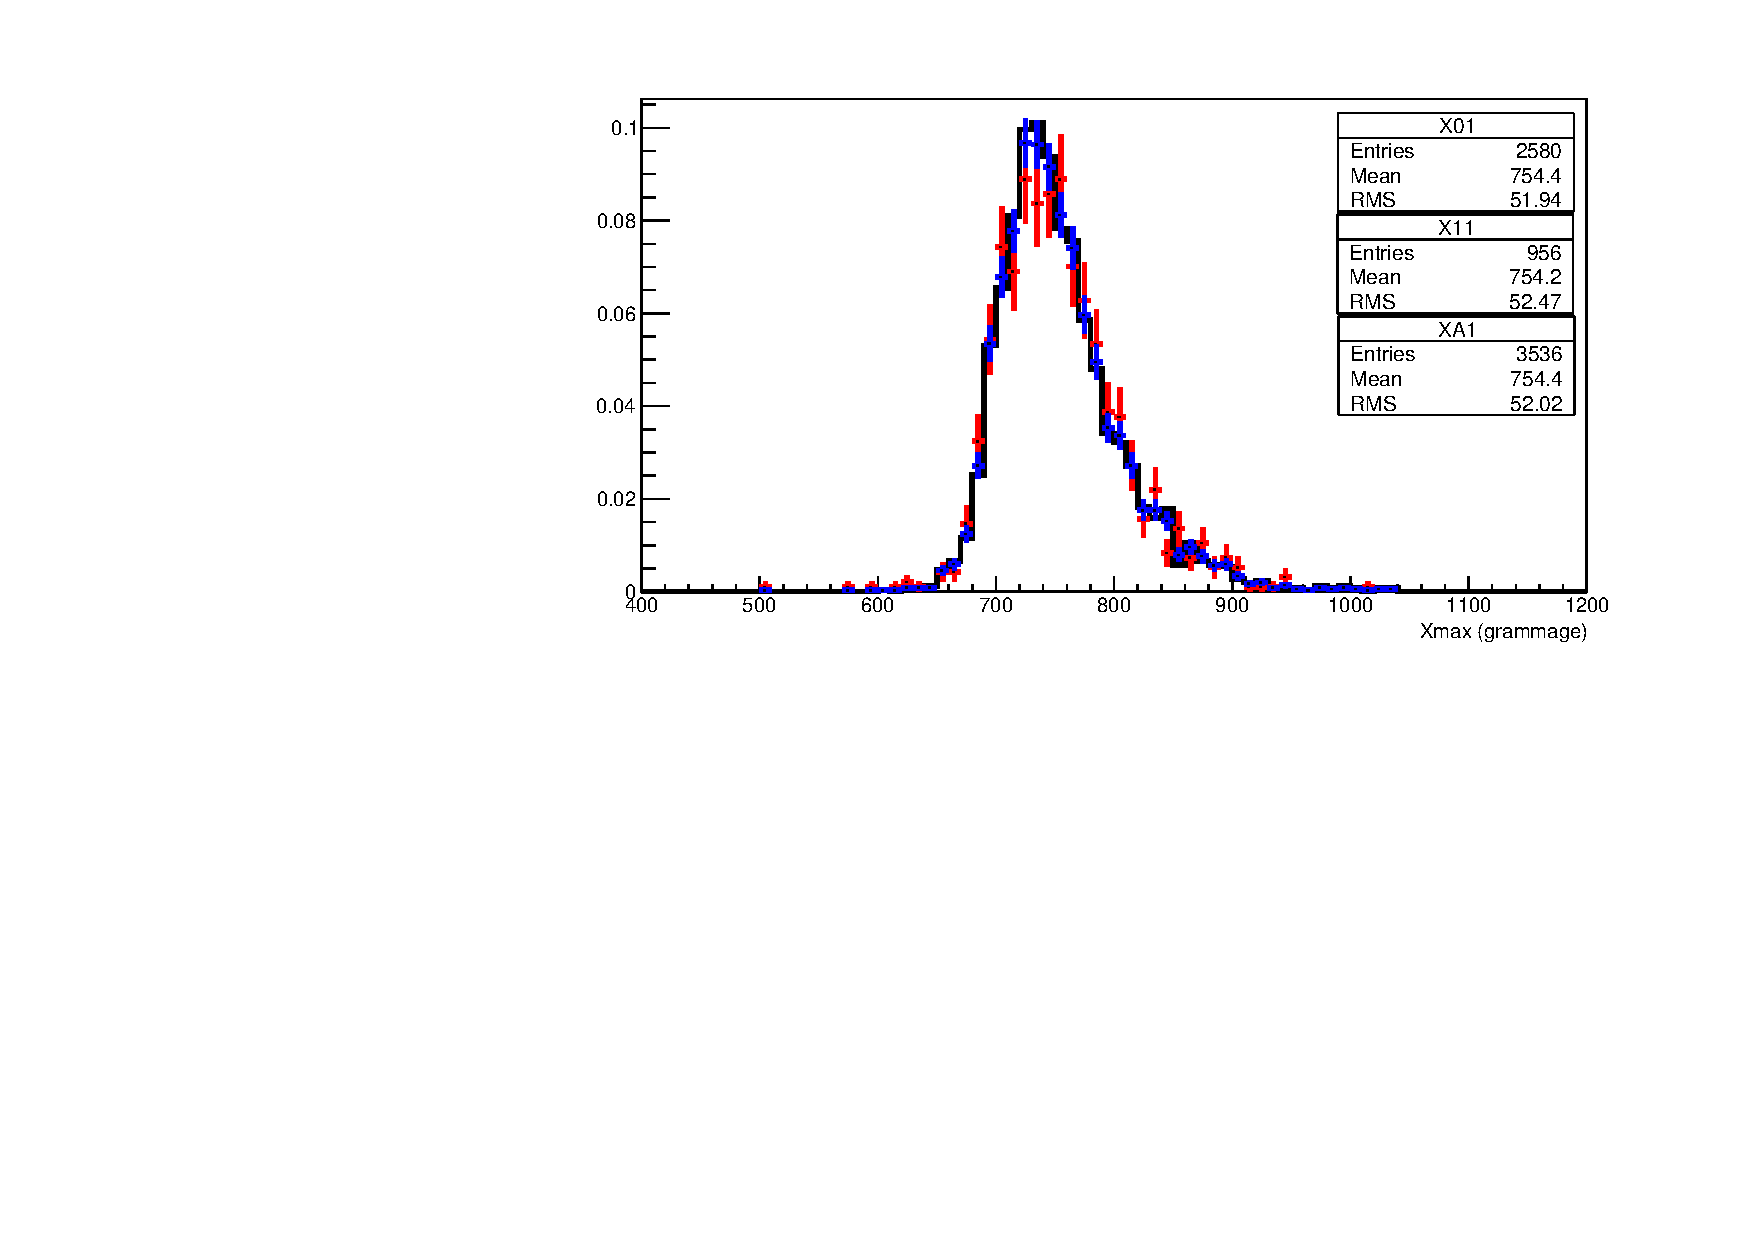
\includegraphics[width=\textwidth]{/home/tsudholz/PhD/Thesis/chapters/graphs/CloudFlags/NormHist_Xmax_logE_18_5to18_75_Comb.pdf}
\caption{Distribution of the Xmax of events within the bin of log(E) of 18.5 to 18.75. Black (XA1) denotes events that passed with cloud cut removed, blue (X01) denotes events that would pass the cloud cuts and red (X11) denotes events that would fail the cloud cuts. All other cuts used for the ICRC19 have been applied.}
\end{figure}

\begin{figure}
\centering
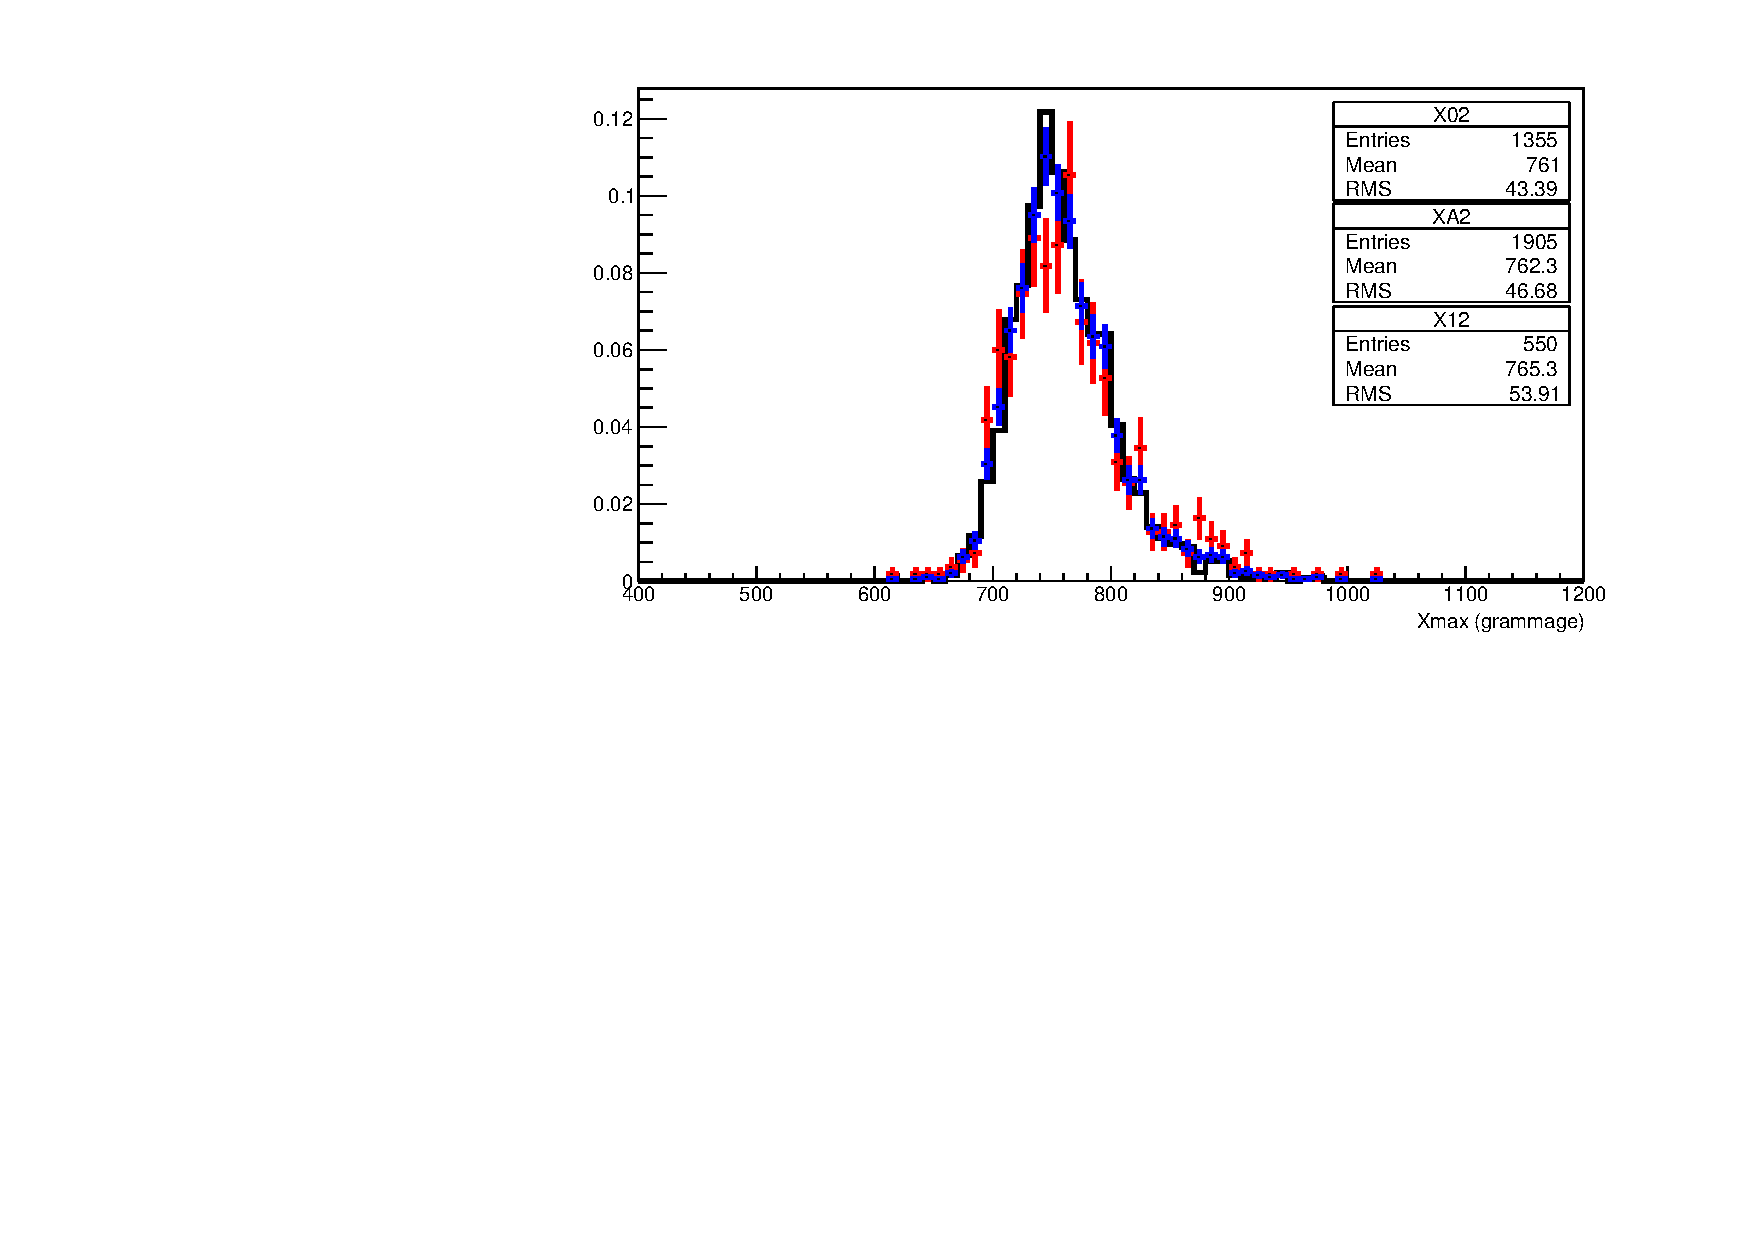
\includegraphics[width=\textwidth]{/home/tsudholz/PhD/Thesis/chapters/graphs/CloudFlags/NormHist_Xmax_logE_18_75to19_0_Comb.pdf}
\caption{Distribution of the Xmax of events within the bin of log(E) of 19.0 to 19.25. Black (XA2) denotes events that passed with cloud cut removed, blue (X02) denotes events that would pass the cloud cuts and red (X12) denotes events that would fail the cloud cuts. All other cuts used for the ICRC19 have been applied.}
\end{figure}

\begin{figure}
\centering
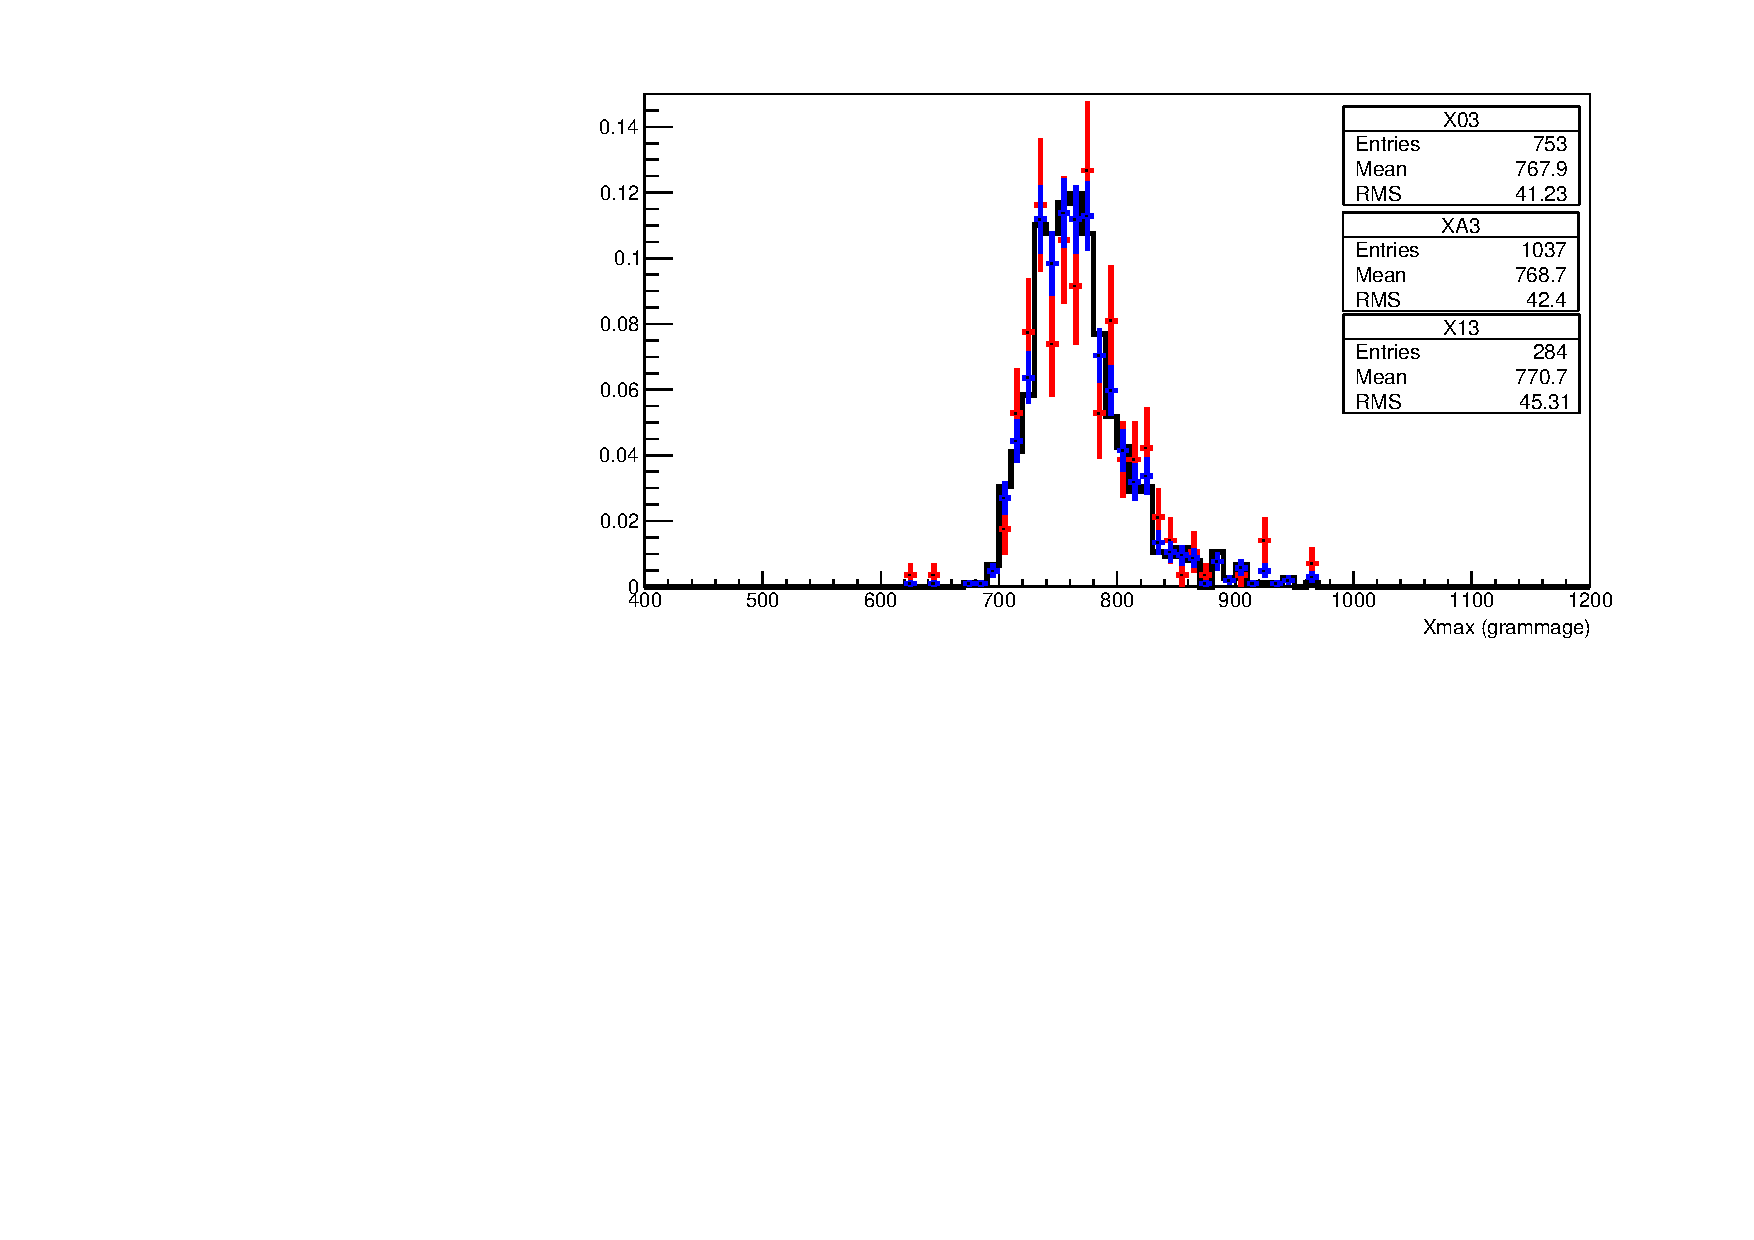
\includegraphics[width=\textwidth]{/home/tsudholz/PhD/Thesis/chapters/graphs/CloudFlags/NormHist_Xmax_logE_19_0to19_25_Comb.pdf}
\caption{Distribution of the Xmax of events within the bin of log(E) of 19.0 to 19.25. Black (XA3) denotes events that passed with cloud cut removed, blue (X03) denotes events that would pass the cloud cuts and red (X13) denotes events that would fail the cloud cuts. All other cuts used for the ICRC19 have been applied.}
\end{figure}

\begin{figure}
\centering
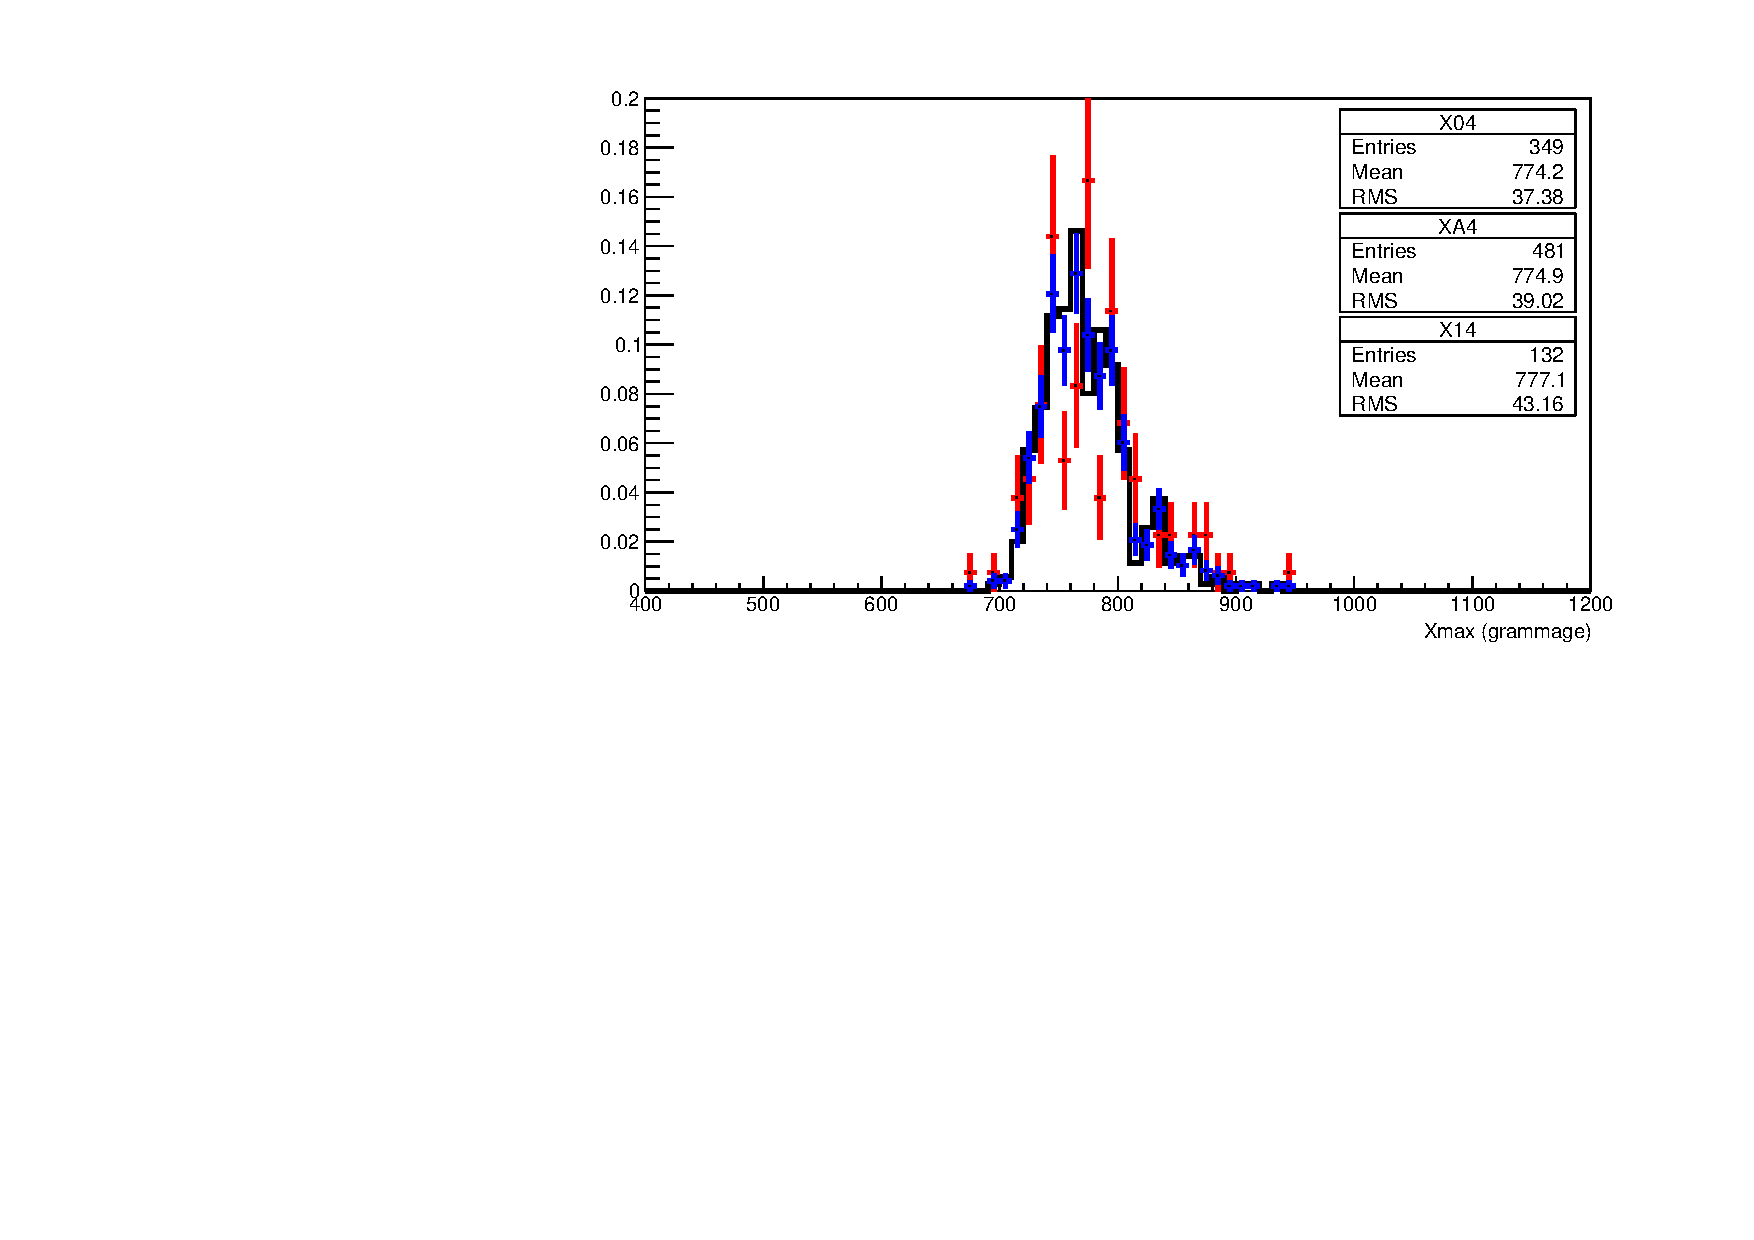
\includegraphics[width=\textwidth]{/home/tsudholz/PhD/Thesis/chapters/graphs/CloudFlags/NormHist_Xmax_logE_19_25to19_5_Comb.pdf}
\caption{Distribution of the Xmax of events within the bin of log(E) of 19.25 to 19.5. Black (XA4) denotes events that passed with cloud cut removed, blue (X04) denotes events that would pass the cloud cuts and red (X14) denotes events that would fail the cloud cuts. All other cuts used for the ICRC19 have been applied.}
\end{figure}

\begin{figure}
\centering
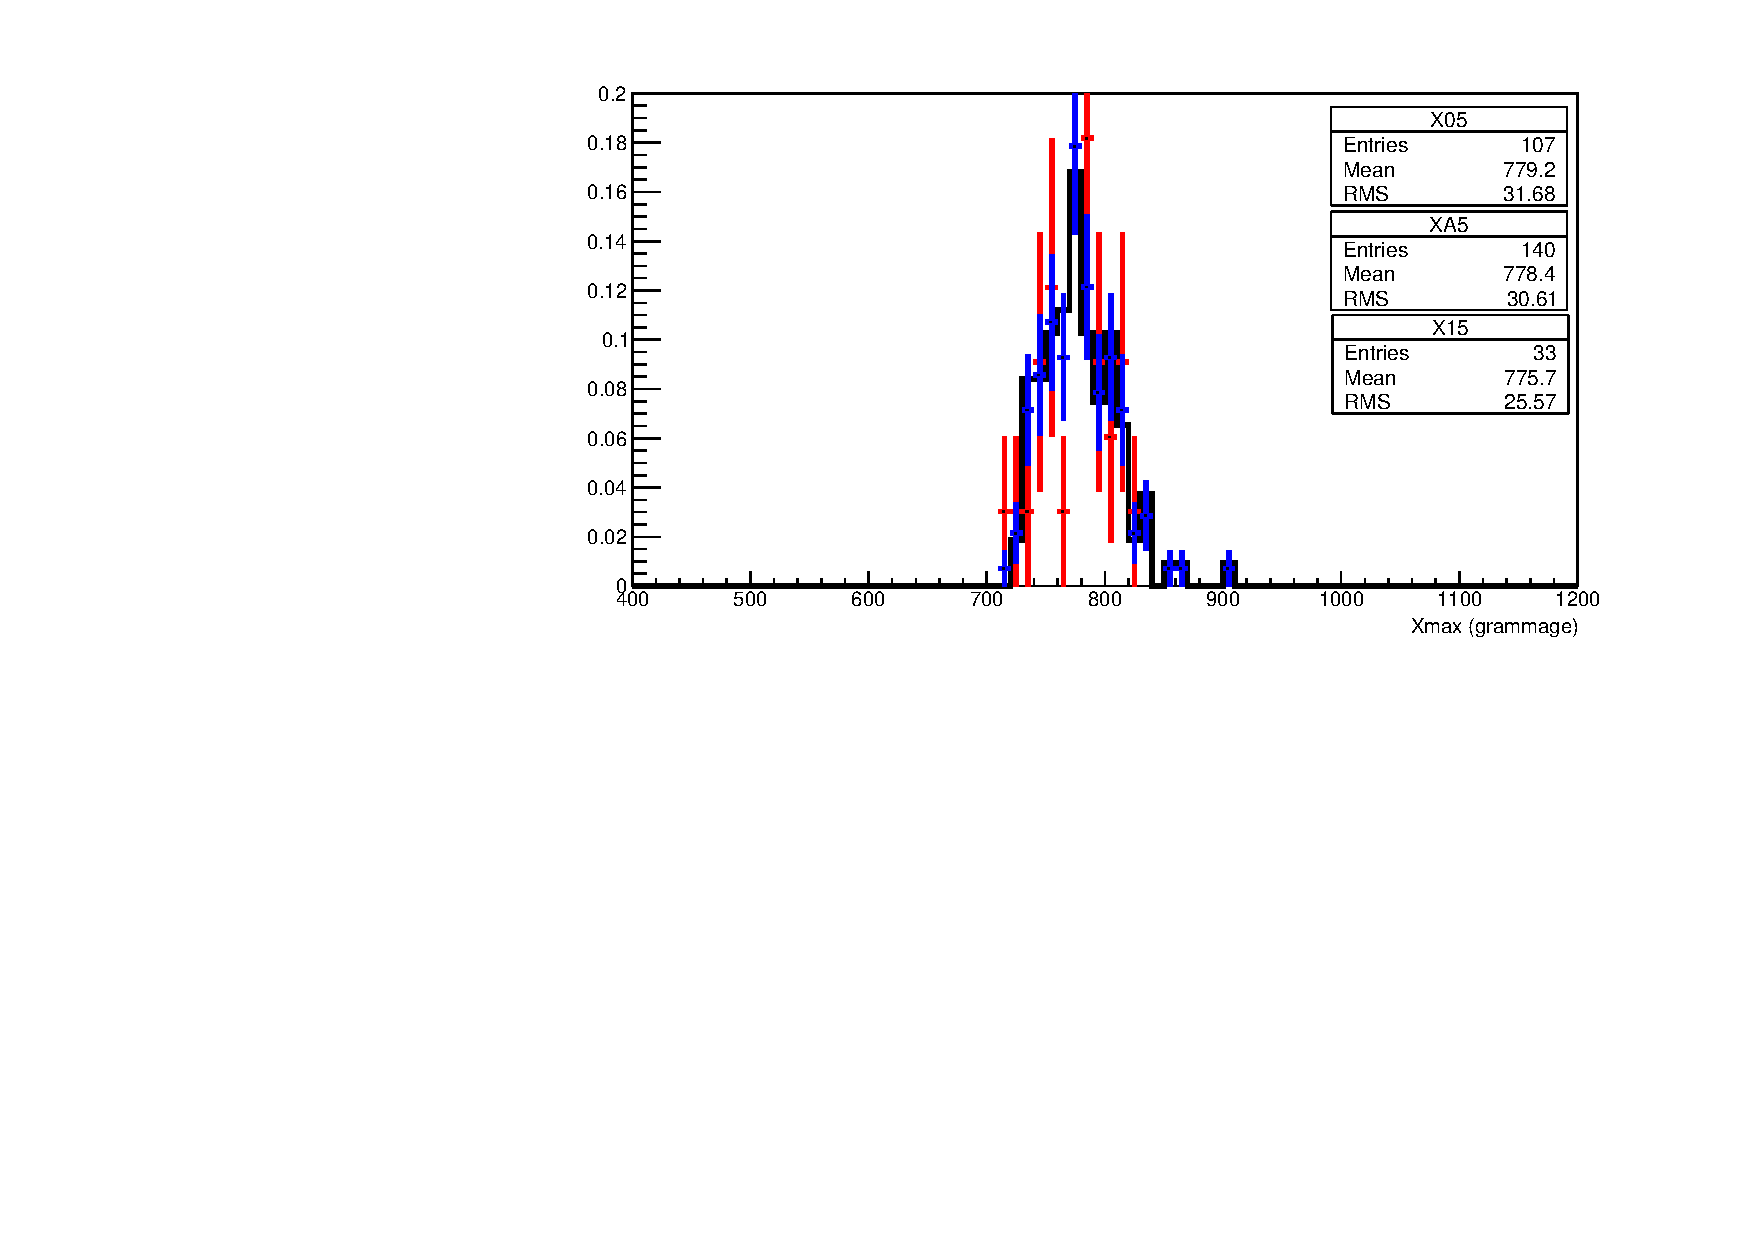
\includegraphics[width=\textwidth]{/home/tsudholz/PhD/Thesis/chapters/graphs/CloudFlags/NormHist_Xmax_logE_Greater19_5_Comb.pdf}
\caption{Distribution of the Xmax of events within the bin of log(E) of greater than 19.5. Black (XA5) denotes events that passed with cloud cut removed, blue (X05) denotes events that would pass the cloud cuts and red (X15) denotes events that would fail the cloud cuts. All other cuts used for the ICRC19 have been applied.}
\end{figure}

% Xmax Distribution for Failed only

\begin{figure}
\centering
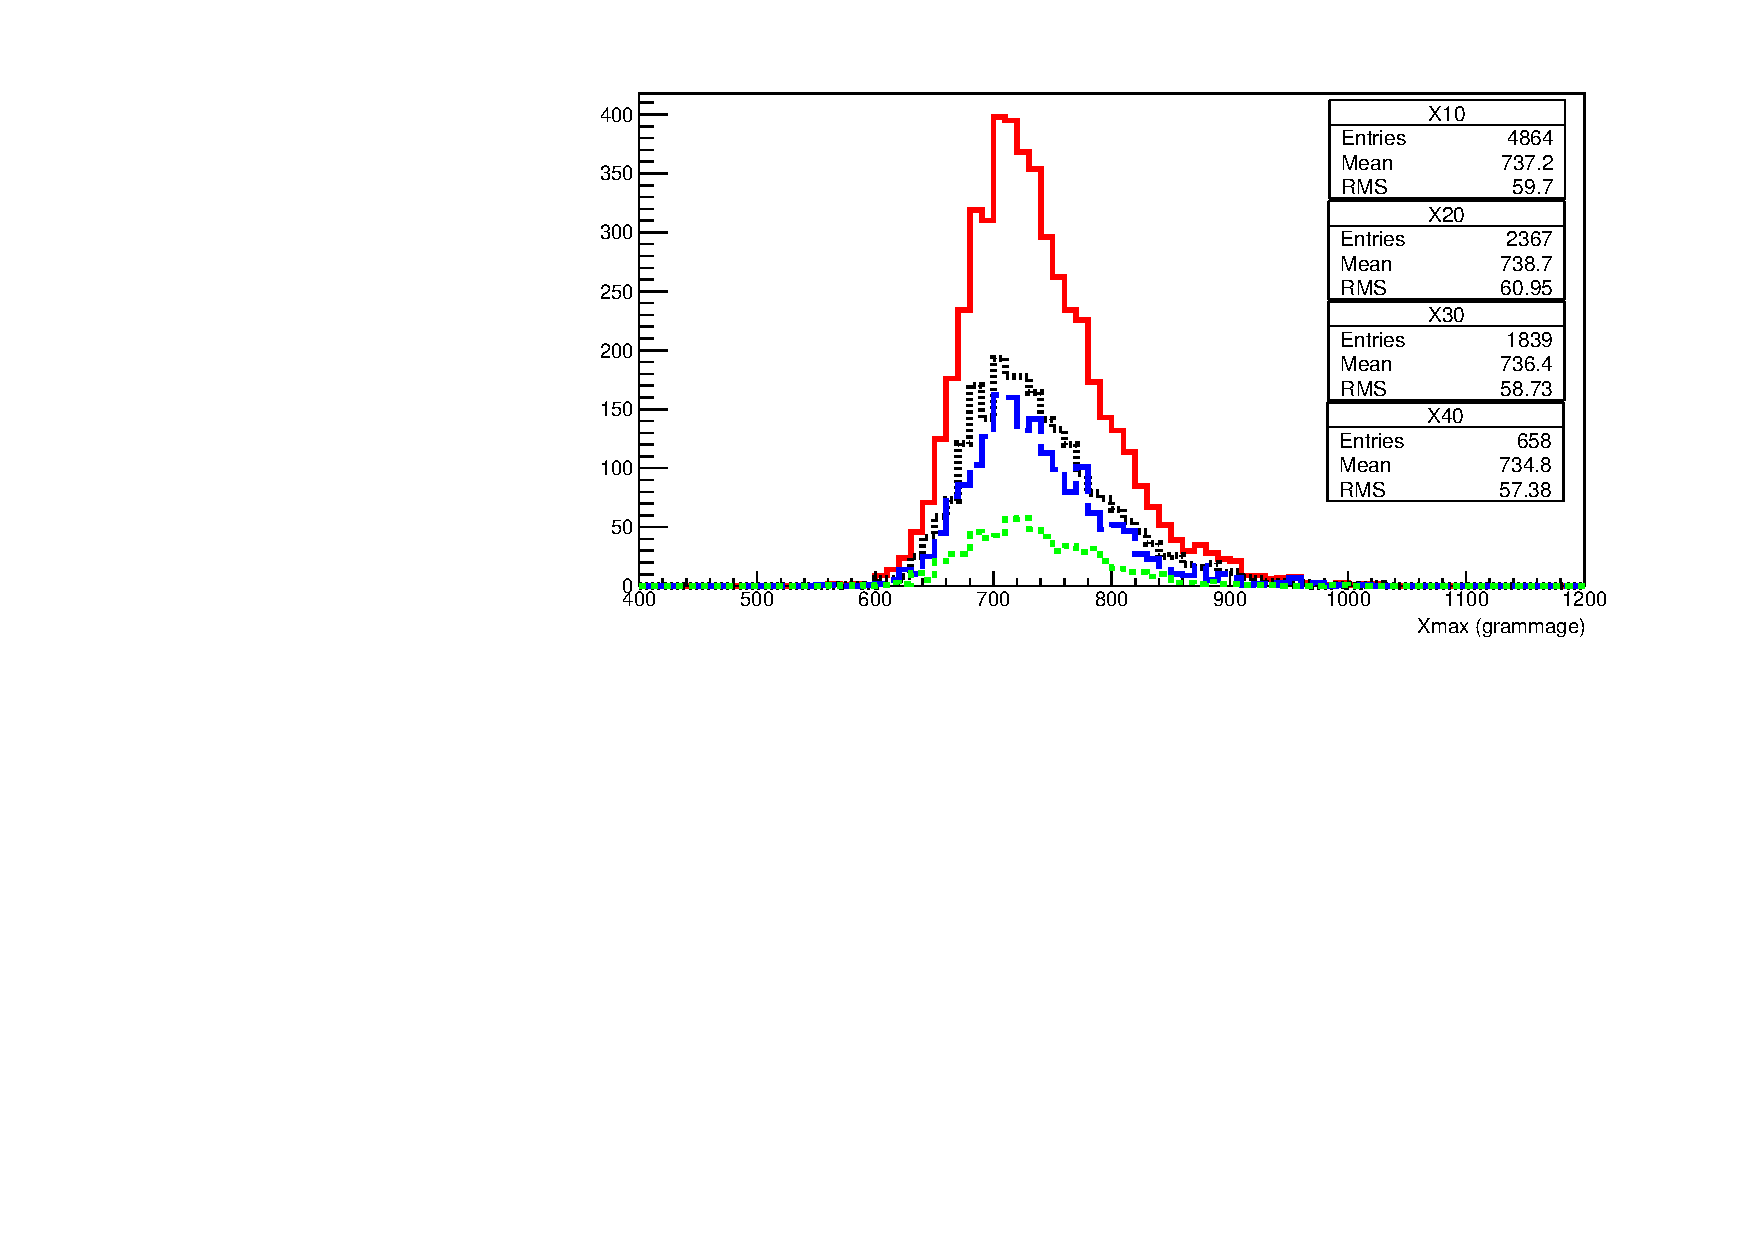
\includegraphics[width=\textwidth]{/home/tsudholz/PhD/Thesis/chapters/graphs/CloudFlags/NormHist_Xmax_FailedCloudCut_logE_18_0to18_5_Comb.pdf}
\caption{Distribution of the energy of events within the bin of log(E) of 18.0 to 18.5. Red (X10) denotes all event that failed the cloud cuts, black (X20) denotes events that failed the cloud camera/lidar cut, blue (X30) denotes events that failed the GOES data cut and green (X40) are events that have fail a combination of CLF/XLF, GOES and Cloud camera cut.}
\end{figure}

\begin{figure}
\centering
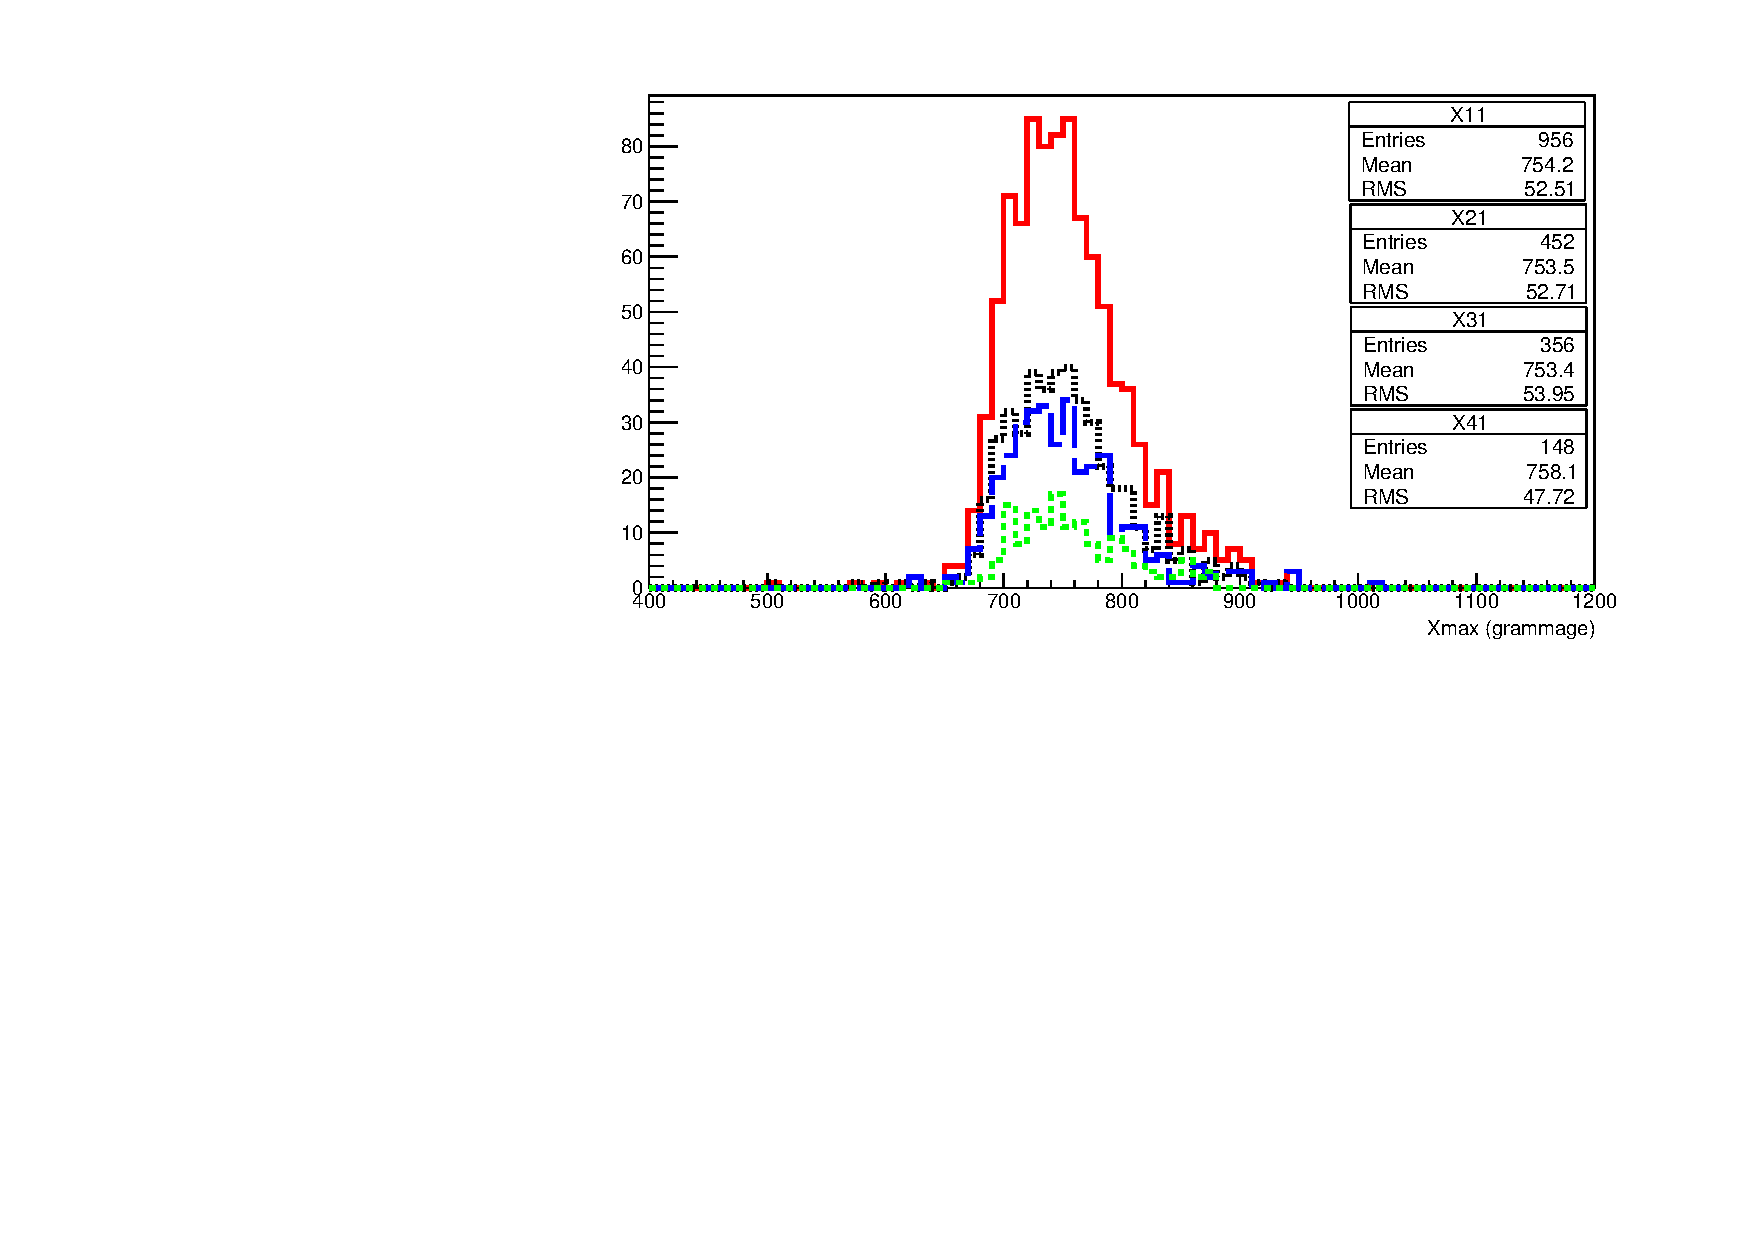
\includegraphics[width=\textwidth]{/home/tsudholz/PhD/Thesis/chapters/graphs/CloudFlags/NormHist_Xmax_FailedCloudCut_logE_18_5to18_75_Comb.pdf}
\caption{Distribution of the energy of events within the bin of log(E) of 18.5 to 18.75. Red (X11) denotes all event that failed the cloud cuts, black (X21) denotes events that failed the cloud camera/lidar cut, blue (X31) denotes events that failed the GOES data cut and green (X41) are events that have fail a combination of CLF/XLF, GOES and Cloud camera cut.}
\end{figure}

\begin{figure}
\centering
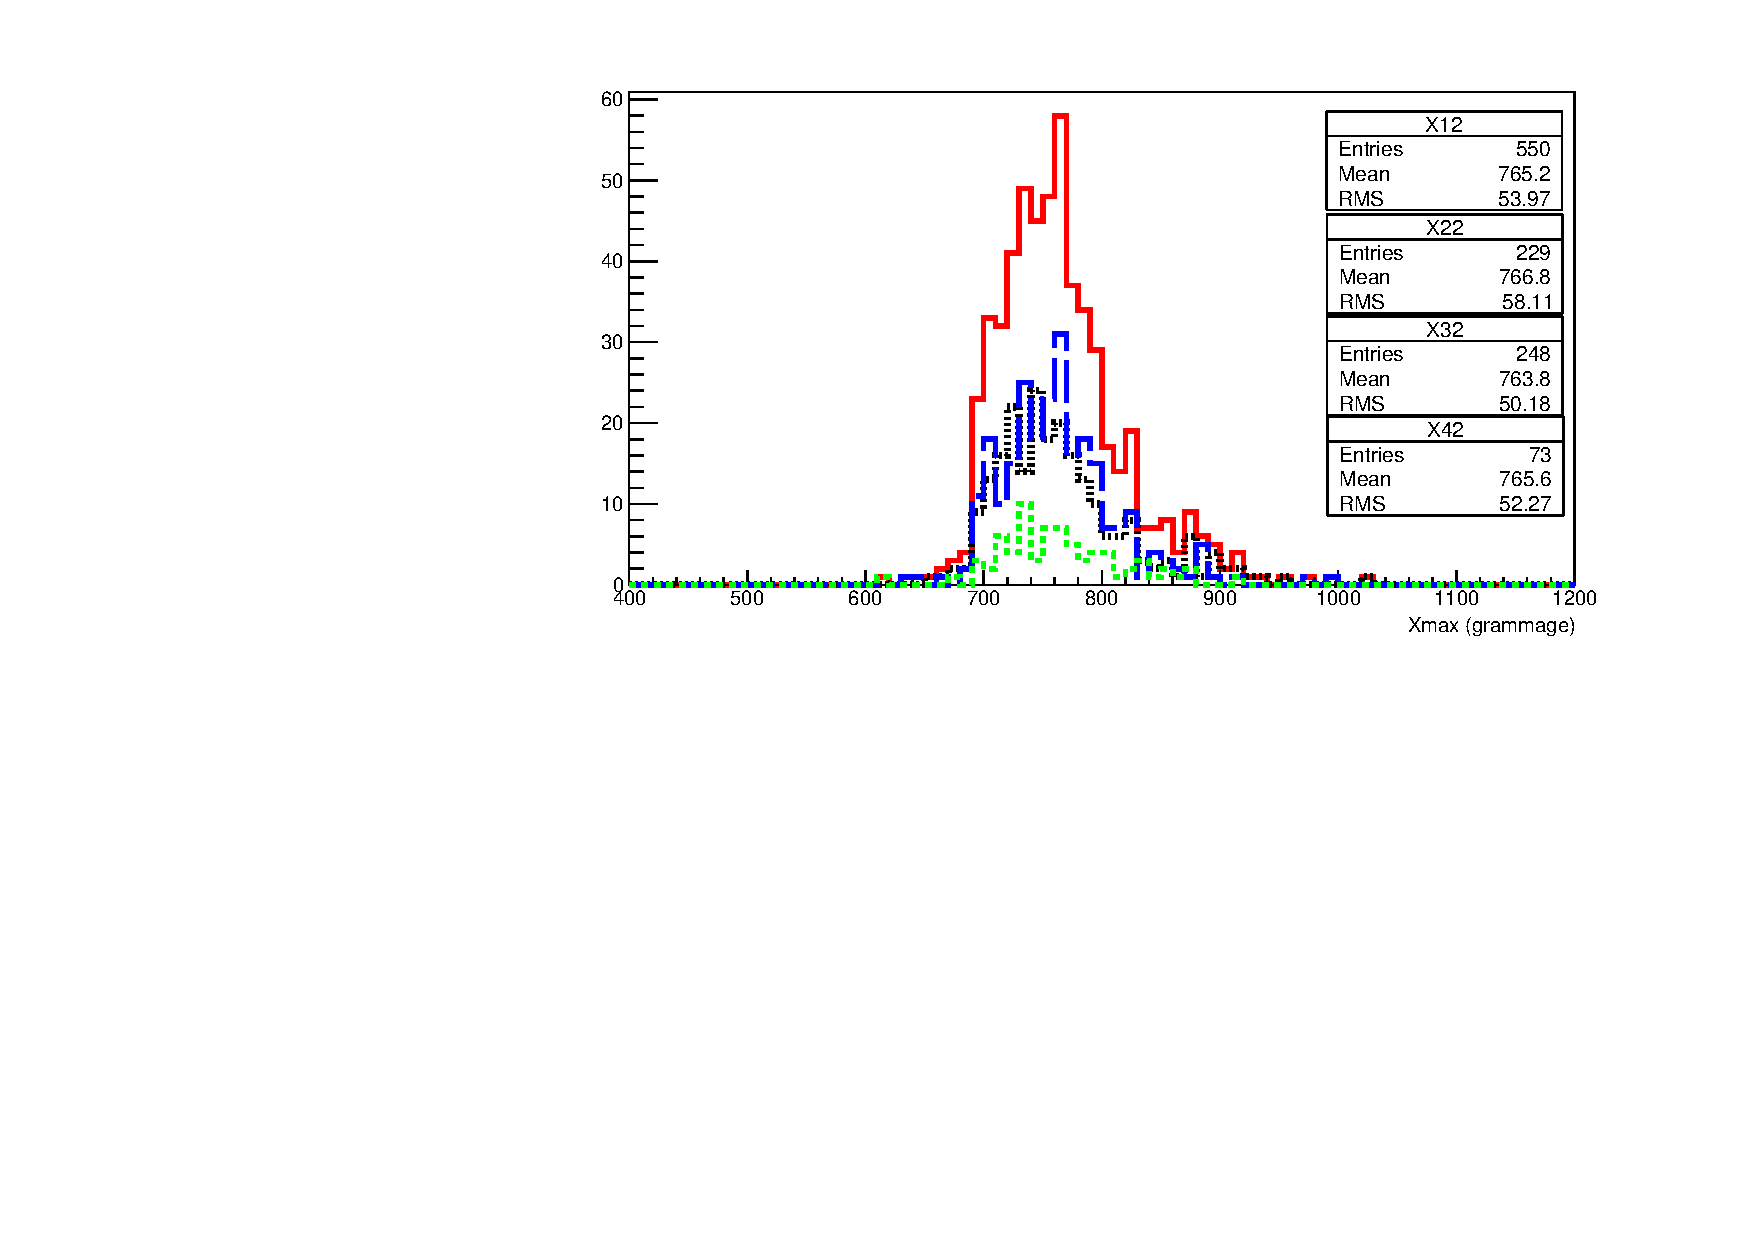
\includegraphics[width=\textwidth]{/home/tsudholz/PhD/Thesis/chapters/graphs/CloudFlags/NormHist_Xmax_FailedCloudCut_logE_18_75to19_0_Comb.pdf}
\caption{Distribution of the energy of events within the bin of log(E) of 18.75 to 19.0. Red (X12) denotes all event that failed the cloud cuts, black (X22) denotes events that failed the cloud camera/lidar cut, blue (X32) denotes events that failed the GOES data cut and green (X42) are events that have fail a combination of CLF/XLF, GOES and Cloud camera cut.}
\end{figure}

\begin{figure}
\centering
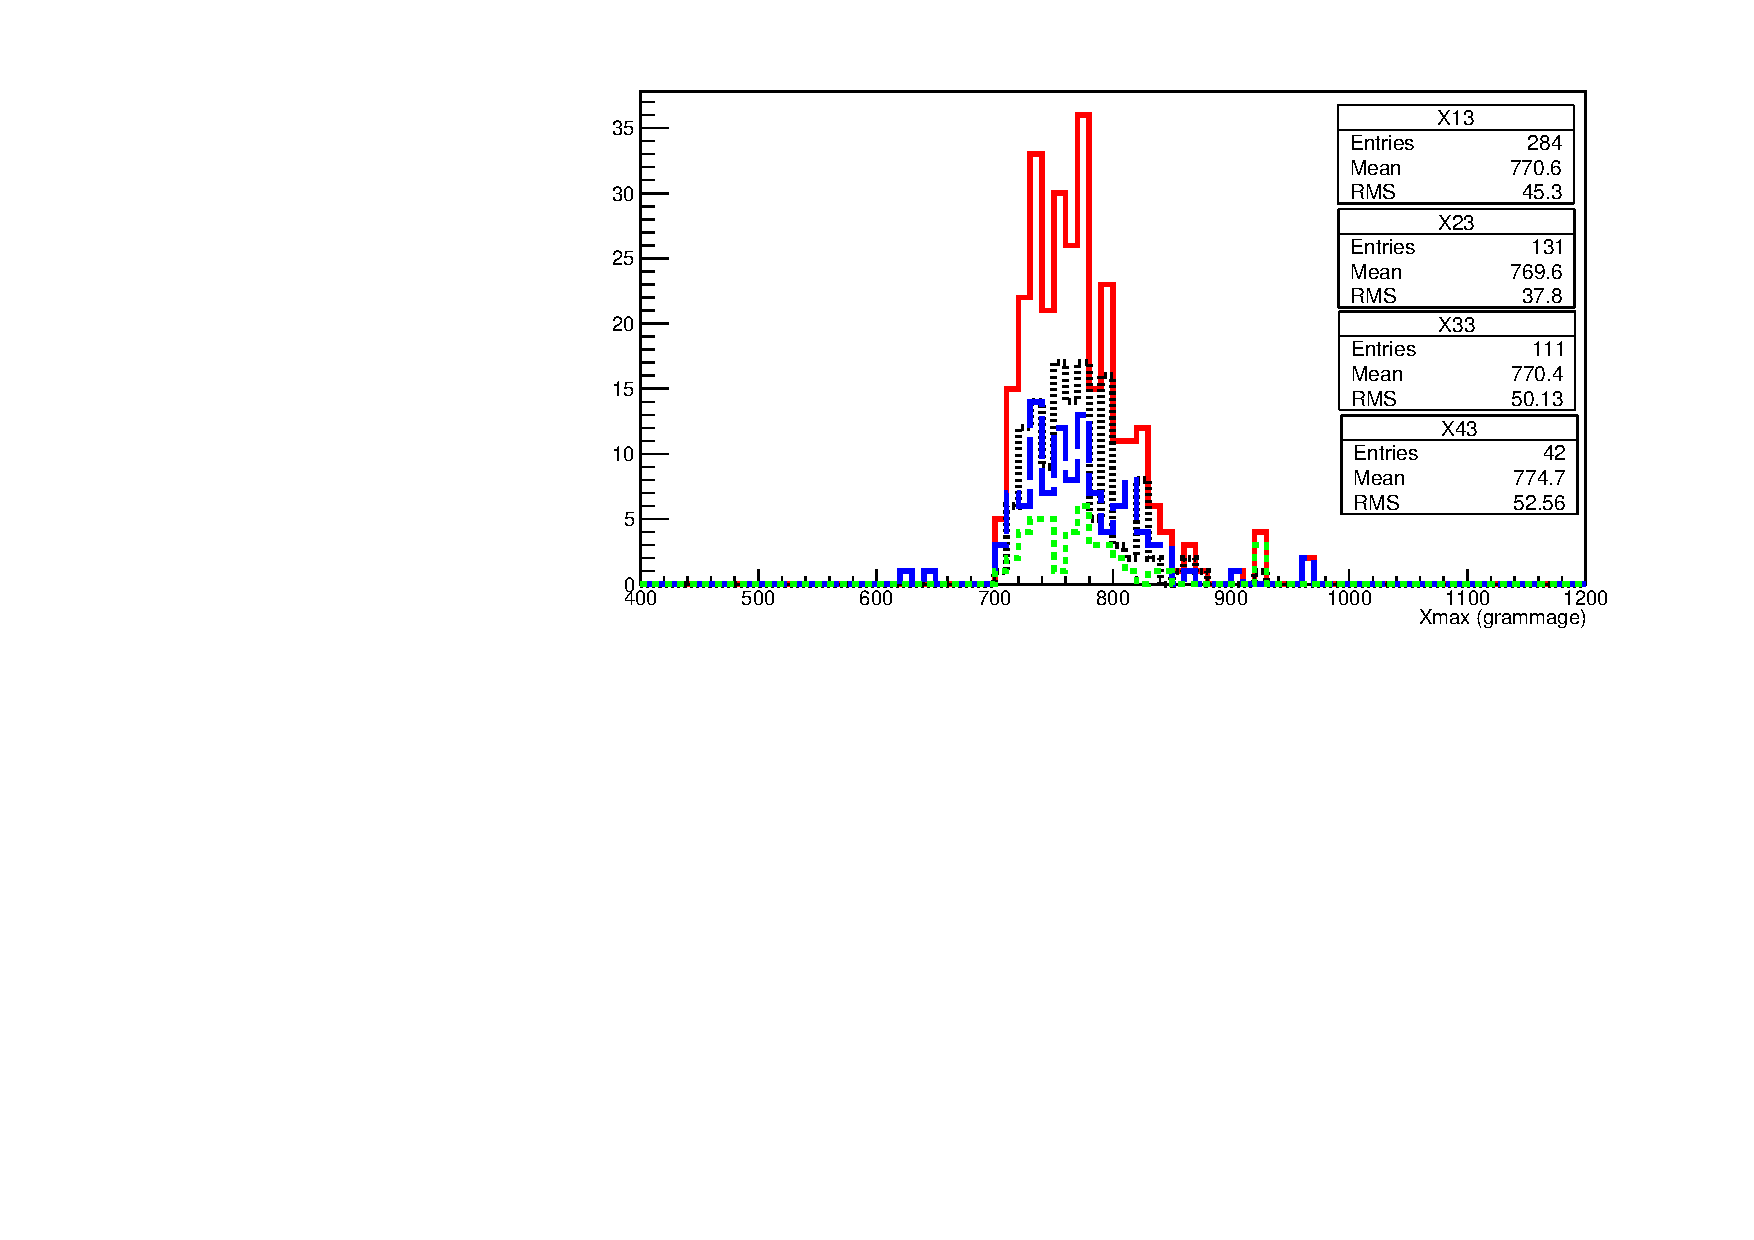
\includegraphics[width=\textwidth]{/home/tsudholz/PhD/Thesis/chapters/graphs/CloudFlags/NormHist_Xmax_FailedCloudCut_logE_19_0to19_25_Comb.pdf}
\caption{Distribution of the energy of events within the bin of log(E) of 19.0 to 19.25. Red (X13) denotes all event that failed the cloud cuts, black (X23) denotes events that failed the cloud camera/lidar cut, blue (X33) denotes events that failed the GOES data cut and green (X43) are events that have fail a combination of CLF/XLF, GOES and Cloud camera cut.}
\end{figure}

\begin{figure}
\centering
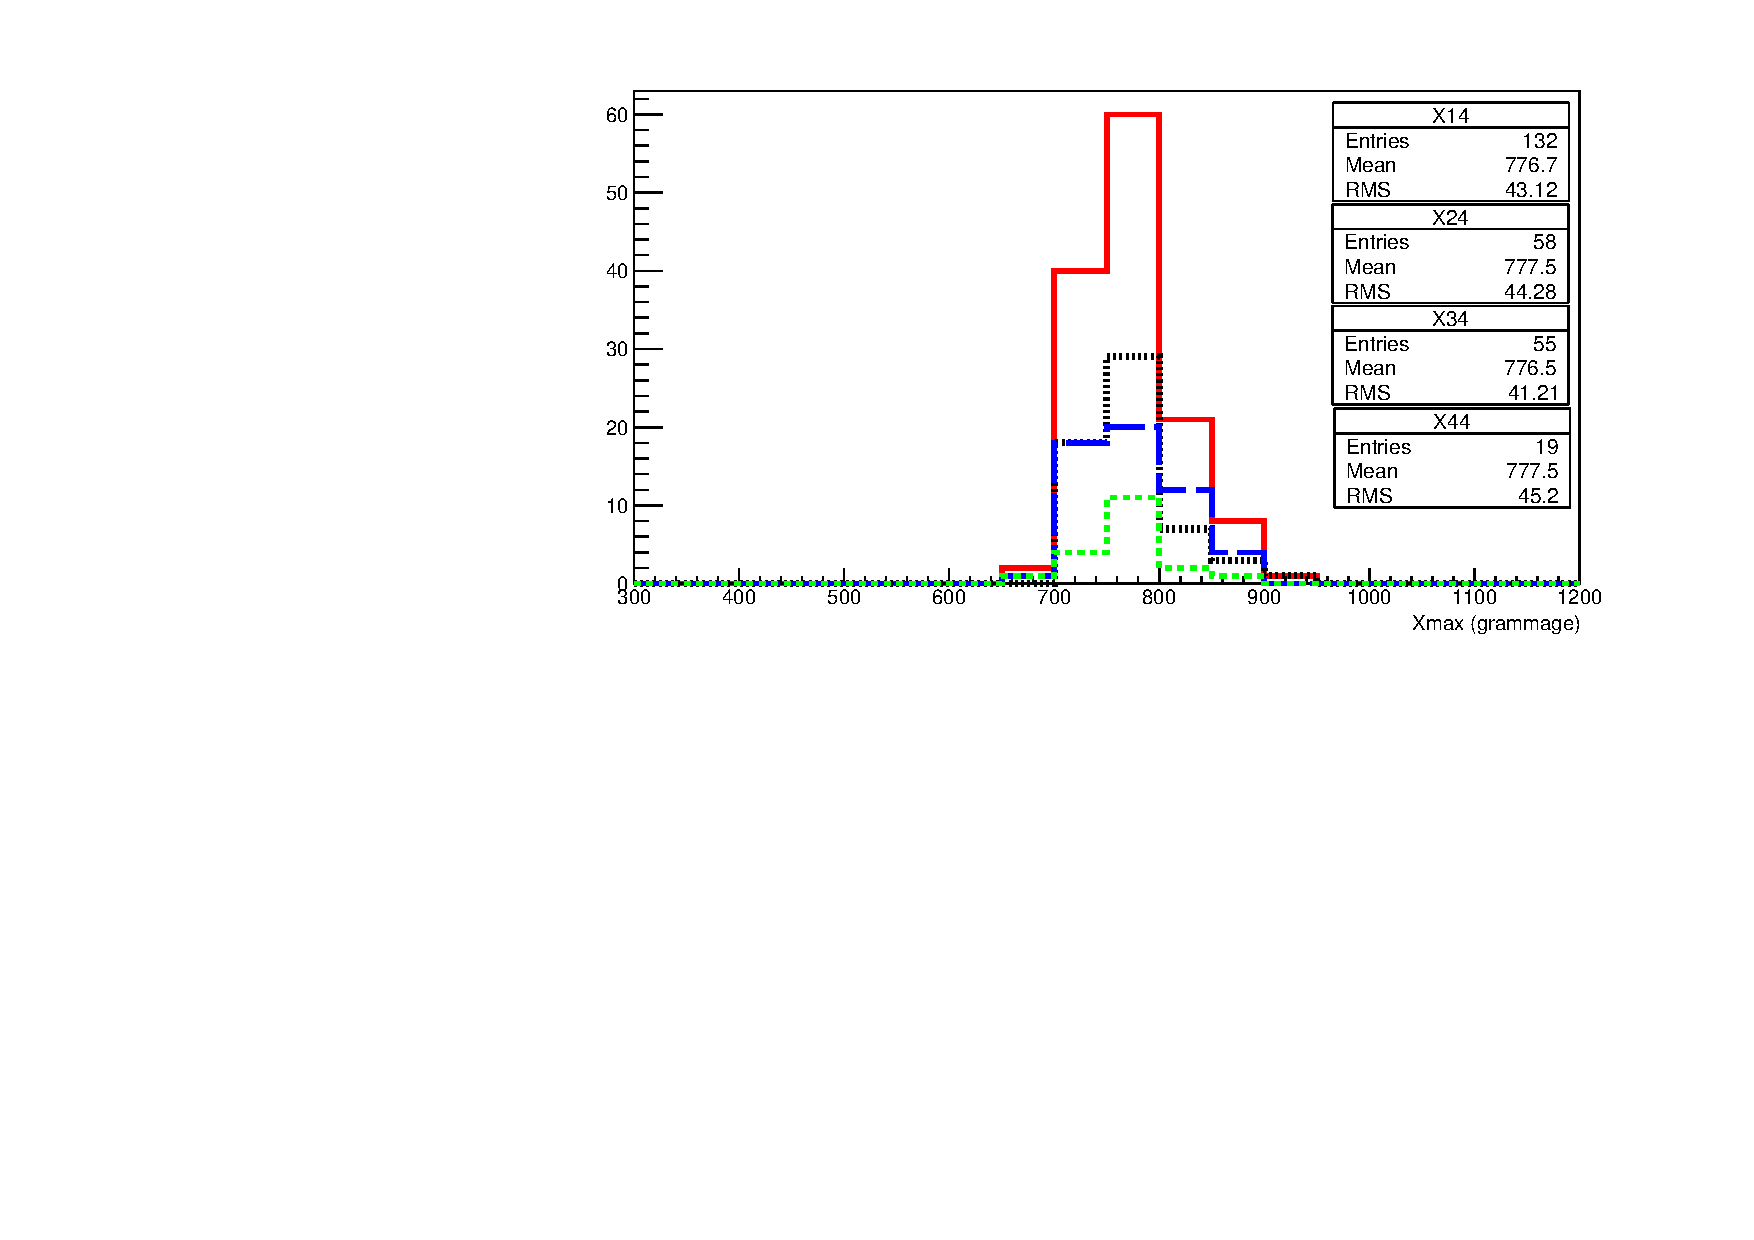
\includegraphics[width=\textwidth]{/home/tsudholz/PhD/Thesis/chapters/graphs/CloudFlags/NormHist_Xmax_FailedCloudCut_logE_19_25to19_5_Comb.pdf}
\caption{Distribution of the energy of events within the bin of log(E) of 19.25 to 19.5. Red (X14) denotes all event that failed the cloud cuts, black (X24) denotes events that failed the cloud camera/lidar cut, blue (X34) denotes events that failed the GOES data cut and green (X44) are events that have fail a combination of CLF/XLF, GOES and Cloud camera cut.}
\end{figure}

\begin{figure}
\centering
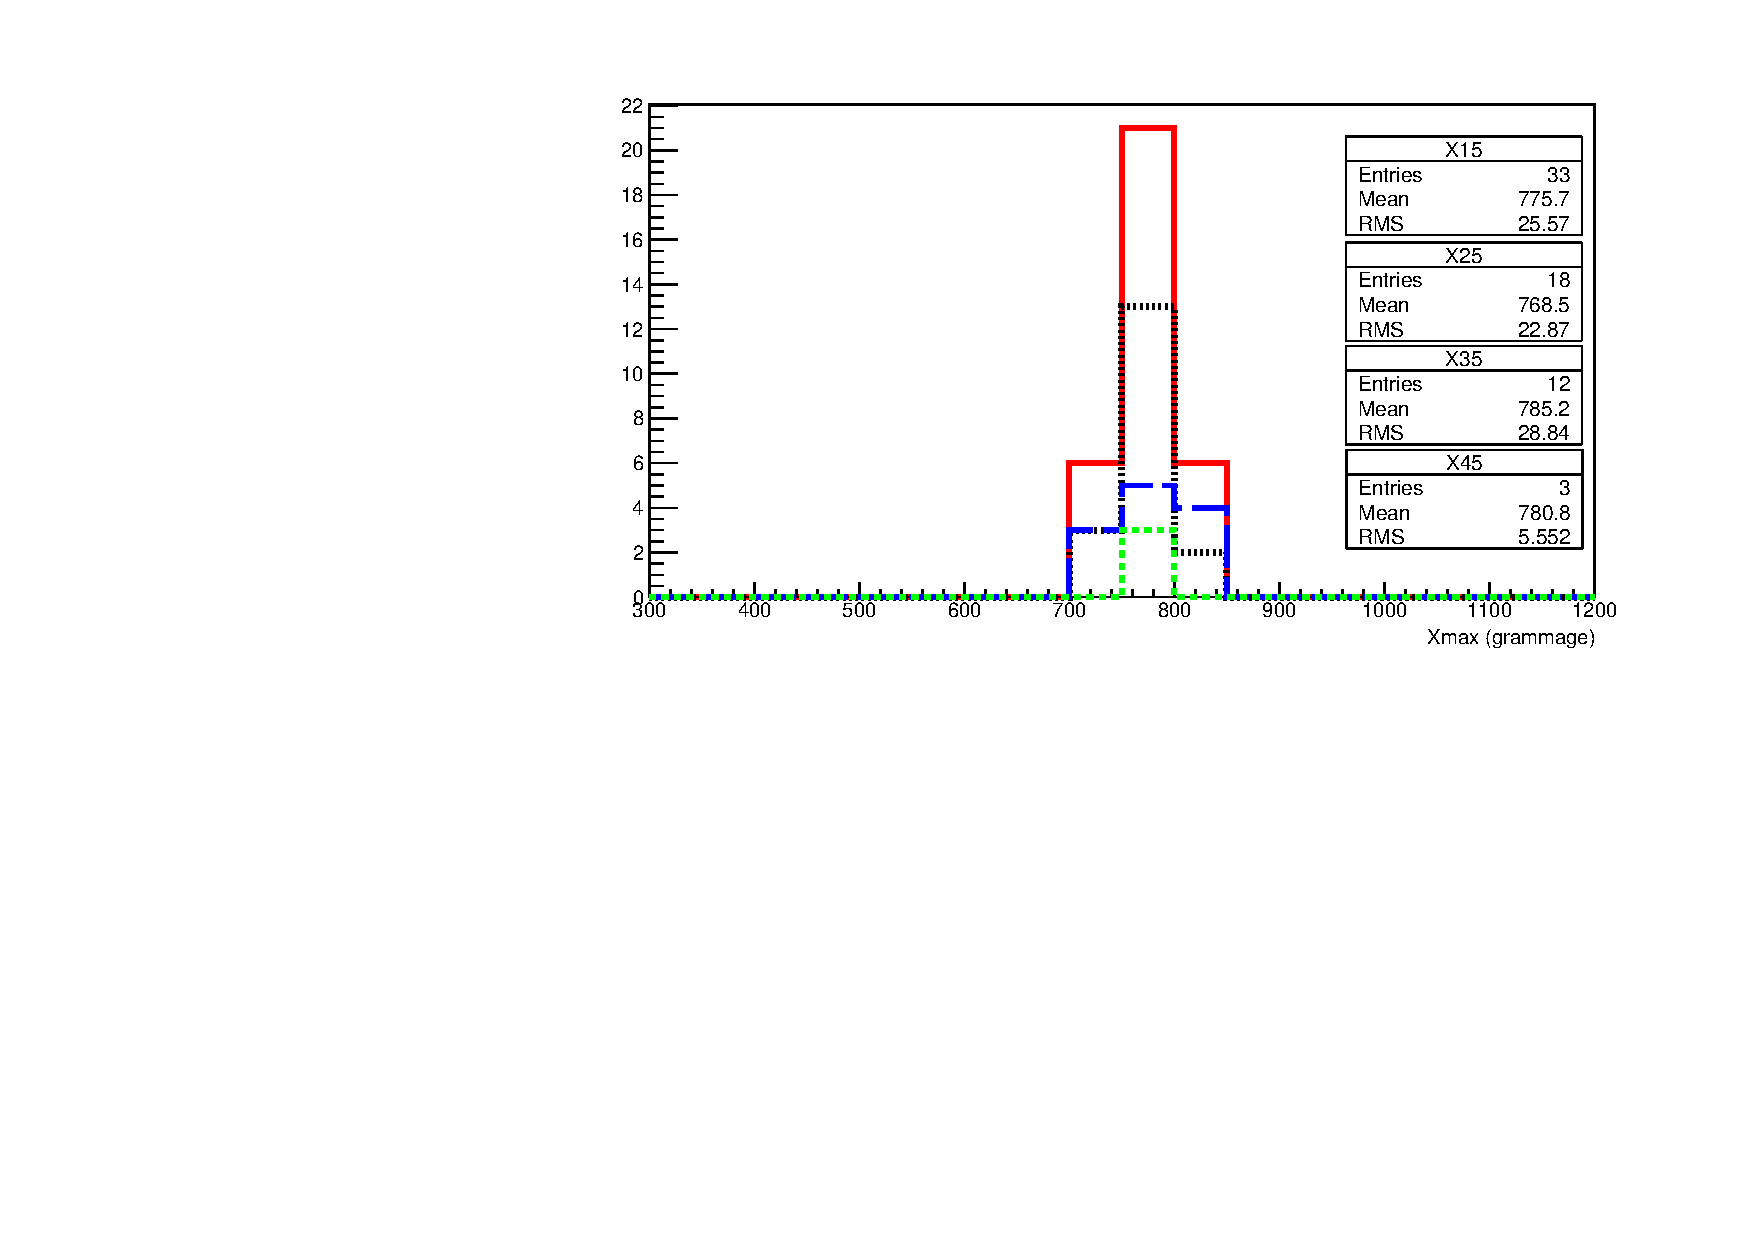
\includegraphics[width=\textwidth]{/home/tsudholz/PhD/Thesis/chapters/graphs/CloudFlags/NormHist_Xmax_FailedCloudCut_logE_Greater19_5_Comb.pdf}
\caption{Distribution of the energy of events within the bin of log(E) of greater than 19.5. Red (X15) denotes all event that failed the cloud cuts, black (X25) denotes events that failed the cloud camera/lidar cut, blue (X35) denotes events that failed the GOES data cut and green (X45) are events that have fail a combination of CLF/XLF, GOES and Cloud camera cut.}
\end{figure}

\section{Discussion - Are we being too conservative?}

Gaining 30\% more events cut is removed

Have to be careful of outliers

Mean Xmax and spread in Xmax does not change significantly

With cloud cut confident that events that could be cloud effected are removed. Without the cloud cut no significant impact is seem expect for the increase of statistics by 30\%.


\section{Conclusion}
